\documentclass[11pt]{article}
\title{ECO325: Lecture Notes \\ \small Advanced Economic Theory: Macro}
\author{Tianyu Du}
\date{\today}

\usepackage{spikey}
\usepackage{amsmath}
\usepackage{amssymb}
\usepackage{soul}
\usepackage{float}
\usepackage{graphicx}
\usepackage{hyperref}
\usepackage{xcolor}
\usepackage{chngcntr}

\counterwithin{equation}{section}
\newcommand{\expat}[2]{\mathbb{E}_{#1}\Big[{#2}\Big]}

\usepackage[
    type={CC},
    modifier={by-nc},
    version={4.0},
]{doclicense}


\begin{document}
    \maketitle
    \doclicenseThis
    \section*{Notes}
    	\texttt{Github Page} \url{https://github.com/TianyuDu/Spikey_UofT_Notes}\\
    	\texttt{Note Page} \url{TianyuDu.com/notes}
    \paragraph{Revisions}
    \begin{itemize}
    	\item Revise October 2. 2018. Midterm 1. Lec1-Lec4
    	\item Revise October 21. 2018. Lec5-Lec6
    	\item Revise November 27. 2018. Lec9
    	\item Revise December 15. 2018. Final Revision 1
    \end{itemize}
    \tableofcontents
    \newpage
    
    \section{Lecture 1 September 6. 2018}
        \begin{definition}
            A \textbf{growth miracle} are episodes where thee growth in a country far exceeds the world average over an extended period of time. \\
            \ul{Result}: the country experiencing the miracle \ul{moves up in the} \hl{wold income distribution}.
        \end{definition}
        
        \begin{definition}
            A \textbf{growth disaster} is an episodes where the growth in a country falls short at the world average for an extended period of time. \\
            \ul{Result}: the country \ul{moves down in the world income distribution}.
        \end{definition}
    
        \paragraph{Economic Growth Facts}(with corresponding result from Solow growth model.)
        \begin{enumerate}
            \item Real output($Y$) grows at a (more or less) constant rate ($n+g$).
            \item Stock of real capital($K$) grows at a (more or less) constant rate($n+g$) (but it grows faster than labor input($L$)($n$).
            \item Growth rates of real output($Y$) and the stock of capital($K$) are about the same. (both $n+g$)
            \item The rate of growth of output per capita($\frac{Y}{L}$) varies greatly across countries. ($g$ varies across countries)
        \end{enumerate}
        
        \subsection{Solow Growth Model (continuous time)}
            \paragraph{Introduction} Solow growth model decomposes the growth in output per capita $\frac{Y}{L}$ into portions accounted for by increase in \ul{inputs}($L, K$) and the portion contributed to increases in \ul{productivity} ($A$).
           
            \begin{notation}
            		In the baseline model we denote $K$ as capital, $L$ as labor and $A$ as technology.
            \end{notation}
            
        \subsubsection{Production Function}
            \begin{remark}
                \st{Harrod-neutral technology here, refer to Uzawa's theorem.}
            \end{remark}
            \begin{definition}
                The \textbf{effective labor input}(total units off effective labor) is defined as $A(t)L(t)$
            \end{definition}
            
            \begin{definition}
                The \textbf{production function} is defined as a real-valued mapping from input factor space to an output level $F: \mc{K} \times \mc{A} \times \mc{L} \to \R_{\geq 0}$:
	            \begin{equation}
                    \textcolor{orange}{Y(t) = F(K(t), A(t)L(t))}
	            \end{equation}
            \end{definition}
            
            \begin{example}
            	    Cobb-Douglas form of production function.
                \begin{equation}
                    Y(t) = K(t)^\alpha (A(t)L(t))^{1 - \alpha},\ \alpha \in (0, 1)
                \end{equation}
            \end{example}
            
            \begin{assumption} The production function is assumed to be \ul{constant return to scale} in $K$ and $AL$.
	            \begin{equation}
	            		Y(cK, cAL) = cY(K, AL),\ \forall c \geq 0
	            \end{equation}
	           
	        \begin{remark}
	        		You need to be able to verify if a given function is constant return to scale (homogeneous to degree one) and choosing parameters to make certain function CRS.
	        \end{remark}
	        
	        \begin{example}
	        		For what values of parameters that production function given below is CRS (i.e. homogeneous to degree 1)
	        		\begin{equation}
	        			Y(t) = K(t)^\alpha (A(t)L(t))^\gamma + C A(t) + B
	        		\end{equation}
	        		\emph{Solution.}
	        		\[
	        			\begin{cases}
	        				\gamma = 1 - \alpha \\
	        				C = 0 \\
	        				B = 0
	        			\end{cases}
	        		\]
	        \end{example}
	            
           	\paragraph{Interpretation} CRS assumption is the result of two separate assumptions.
           	\begin{enumerate}
           		\item \emph{The economy is big enough that the gains from specialization have been exhausted.} $\implies$ There is \textbf{no} increasing return to scale.
           		\item \emph{Inputs other than capital, labor, and the effectiveness of labor are relatively unimportant.} $\implies$ There is \textbf{no} decreasing return to scale.
           	\end{enumerate}
            \end{assumption}
            
            \begin{definition}
                Define $c := \frac{1}{AL}$, the \textbf{intensive form of production function} is
                \begin{equation}
                    y(t) = \frac{Y(t)}{A(t)L(t)} = f(k(t))
                \end{equation}
                where $y := \frac{Y}{AL}$ denotes the output \emph{per unit of effective labor} and $k := \frac{K}{AL}$ denote the capital stock per unit of effective labor.
            \end{definition}
	
	\section{Lecture 2 September 13. 2018}
		\subsection{Solow Growth Model: Setup}
			\begin{definition}
				\textbf{Production function} $F: \R^2_{+} \rightarrow \R_+$ maps input factors:
				\begin{itemize}
					\item $K(t) := $ aggregate capital stock at time $t$.
					\item $L(t) := $ aggregate labor supple at time $t$.
					\item $A(t) := $ \ul{effectiveness} \footnote{Also called labor-argumented technology or Harrod-neutral technology} of labor at time $t$.
				\end{itemize} 
				to output values ($Y(t) := $ aggregate output at time $t$.) The production function takes the form of
				\begin{equation}
					Y(t) = F(K(t), A(t)L(t))
				\end{equation}
			\end{definition}
			
			\begin{assumption}[Assumptions on Production Function]
				The production function are assumed to be \ul{constant return to scale} in $A(t)L(t)$ and $K(t)$.
				\begin{equation}
					cF(K(t), A(t)L(t)) = F(cK(t), cA(t)L(t)),\ \forall c > 0
				\end{equation}
			\end{assumption}
			
			\begin{remark}
				We assume CRS property on the \emph{aggregate} production function \emph{only}, but the intensive-form production generally experiences increasing return to scale by Inada Condition.
			\end{remark}
			
			\begin{definition}
				The \textbf{intensive form of production function} is defined as the output per unit of effective labor. \\
				Let 
				\begin{equation}
					f(t) := \frac{Y(t)}{A(t)L(t)}
				\end{equation}
				and 
				\begin{equation}
					k(t) := \frac{K(t)}{A(t)L(t)}
				\end{equation}
				denote the output and capital per unit of effective labor respectively. By the assumption of \emph{CRS} on \emph{aggregate} production function, take $c = \frac{1}{A(t)L(t)}$. The \emph{intensive form} production function can be expressed as
				\begin{equation}
					\textcolor{orange}{
						y(t) = f(k(t))
					}
				\end{equation}
			\end{definition}
			
			\begin{assumption}[Assumptions on Intensive Form Production Function] the function $f(\cdot): \R_+ \rightarrow \R_+$ is assumed to satisfy \textbf{Inada Conditions}.
				\begin{enumerate}
					\item $f(0) = 0$: capital is necessary for production.
					\item $f'(k) > 0,\ \forall k \in \R_+$: the marginal return of capital per effective unit of labor is positive.
					\item $f''(k) < 0,\ \forall k \in \R_+$: capital per effective unit of labor is experiencing diminishing marginal return.
					\item $\lim_{k \to 0}f'(k) = \infty$
					\item $\lim_{k \to \infty}f'(k) = 0$
				\end{enumerate}
			\end{assumption}
			
			\begin{remark}	
			The role of assumption 2.2 is to ensure that the path of the economy does not diverge.
			\end{remark}
			
			\begin{example}[Cobb-Douglas Production Function is CRS and follows Inada Conditions]
				Consider the Cobb-Douglas production function
				\begin{equation}
					Y(t) = K(t)^\alpha (A(t)L(t))^{1 - \alpha},\ \alpha \in (0, 1)
				\end{equation}
				
				\begin{proof}
					Let $c \in \R_+$, 
					\begin{gather}
						F(cK, cAL) = (cK)^\alpha (cAL)^{1 - \alpha} \\
						= c^\alpha c^{1-\alpha} K^\alpha AL^{1-\alpha} \\
						= cK^{\alpha} AL^{1-\alpha} = cF(K, AL)
					\end{gather}
					CRS on aggregate form is shown. \\
					Notice that $f(k) = k^{\alpha}$ \\
					And 
					\begin{enumerate}
						\item $f(0) = 0^{\alpha} = 0$
						\item $f'(k) = \alpha k ^ {\alpha - 1} > 0, \forall k \in \R_+$
						\item $f''(k) = (\alpha - 1)\alpha k ^ {\alpha - 2} < 0, \ \forall k \in \R_+$
						\item $\lim_{k \to 0} \alpha \frac{1}{k^{1-\alpha}} = \infty$
						\item $\lim_{k \to \infty} \alpha \frac{1}{k^{1-\alpha}} = 0$
					\end{enumerate}
					Inada conditions on intensive form are shown. \\
				\end{proof}
			\end{example}
			
			\begin{assumption}[Assumptions on the Economy]
				Assume the initial values of $K, A, L$ are given and strictly positive. Labor and Knowledge are assumed to grow at an exogenously given constant rate, denoted as $n, g$ respective.
				\begin{gather}
				\textcolor{orange}{
					\dot{L}(t) = nL(t),\ n > 0 }\\
					\textcolor{orange}{
						\dot{A}(t) = gA(t),\ g > 0
					}
				\end{gather}
			\end{assumption}
			
			\begin{proposition}
				Notice the \ul{growth rate} of variable $X(t)$ is given by 
				\[
					g_X := \frac{\dot{X(t)}}{X(t)} = \pd{\ln{X(t)}}{t}
				\]
			\end{proposition}
			\begin{proof}
				\begin{gather}
					\pd{\ln{X(t)}}{t} = \pd{\ln{X(t)}}{X(t)} \pd{X(t)}{t} \\
					= \frac{1}{X(t)} \dot{X(t)}
					= \frac{\dot{X(t)}}{X(t)}
					= g_X \\
				\end{gather}
			\end{proof}
			
			\begin{proposition}
				The functional form of technology and labor at time $t$ can be found by solving ODEs 
				\begin{gather}
					\textcolor{orange}{
						L(t) = e^{nt} L(0)
						} \\
					\textcolor{orange}{
						A(t) = e^{gt} A(0)
						}
				\end{gather}
			\end{proposition}
			
			\begin{assumption}
				Assume there is \emph{no government} and the Solow economy is a \emph{closed economy}. The output is divided between \emph{consumption} and \emph{investment} as 
				\begin{equation}
					Y(t) = C(t) + I(t)
				\end{equation}
			\end{assumption}
			\par And given $\delta$ as depreciation rate of capital, in discrete time (let $\Delta t = 1$)w e have 
			\begin{gather}
				K_{t+1} = (1-\delta)K_t + I_t \\
				\iff I_t = (K_{t+1} - K_t) + \delta K_t \\
				\tx{As } \Delta \to 0 \tx{ (convert to continuous time)}\\
				\textcolor{orange}{I(t) = \dot{K}(t) + \delta K(t)}
			\end{gather}
			
			\begin{assumption}
				Assume investment equals saving and a \ul{constant friction} $s \in [0, 1]$ of output is saved at each time period $t$. The marginal propensity to save, $s$ is given exogenously.
			\end{assumption}
			
			\par Therefore,
			\begin{gather}
				I(t) = sY(t) \implies \dot{K}(t) + \delta K(t) = sY(t) \\
				\implies \textcolor{orange}{
					\dot{K}(t) = sY(t) - \delta K(t)
					}
			\end{gather}
			
			\subsection{Dynamics of $k(t)$}
				\par For simplicity, assuming $n, g, \delta > 0$ and the dynamics of capital per effective unit of labor follows: 
				\begin{gather}
					\dot{k}(t) := \pd{k(t)}{t} = \pd{}{t} \frac{K(t)}{A(t)L(t)} \\
					= \frac{\dot{K}AL - K(\dot{A}L + A\dot{L})}{(AL)^2} \\
					= \frac{\dot{K}}{AL} - \frac{K\dot{A}L}{(AL)^2} - \frac{K A\dot{L}}{(AL)^2} \\
					= \frac{sY - \delta K}{AL} - \frac{\dot{A}}{A}\frac{K}{AL} - \frac{\dot{L}}{L} \frac{K}{AL} \\
					= sy(t) - (n + g + \delta) k(t)
				\end{gather}
				Where \[s y(t)\] is the \textbf{actual investment} \emph{per unit of effective labor} and \[(n + g + \delta) k(t)\] is the \textbf{break-even investment} per unit of effective labor.
				
				\begin{remark}
					The \textbf{convergence speed} is \ul{inversely} correlated with the value of $| k(t) - k^* |$, where $k^*$ denotes the steady state level of capital stock per effective unit of labor.
				\end{remark}
				
				\begin{remark}
					\textcolor{blue}{
					With \ul{convex} production function ($f''(k) > 0$), then $k(t) < k^* \implies \dot{k} < 0$ and $k(t) > k^* \implies \dot{k} > 0$. The steady state value $k^*$ is \ul{steady but not stable} (with $k(t) \neq k^*$, $k$ does not automatically converge to $k^*$).
					}
				\end{remark}
				\begin{figure}[H]
					\centering
					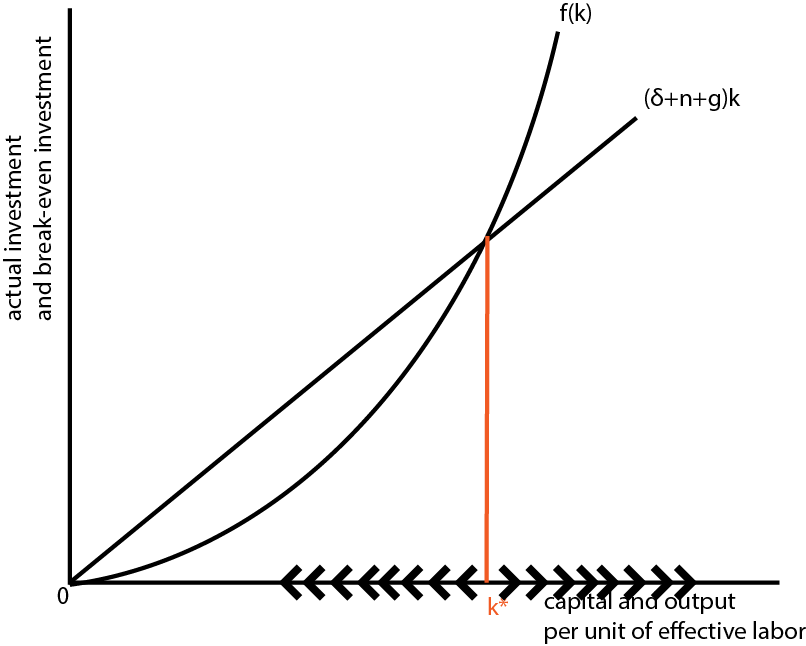
\includegraphics[width=0.7\linewidth]{figures/convex_prod_func.png}
					\caption{A Convex Intensive Form Production Function}
				\end{figure}
	
	\section{Lecture 3 September 20. 2018}
		\subsection{Dynamic Transitions}
			\begin{remark}
				For the dynamic transition function of capital per unit of effective labor:
				\begin{equation}
				\textcolor{orange}{
					\dot{k}(t) = sf(k(t)) - (n+g+\delta)k(t)
					}
				\end{equation}
			\end{remark}
			\paragraph{} And dynamic transition and phase diagram can be expressed as
			\begin{figure}[h]
				\centering
				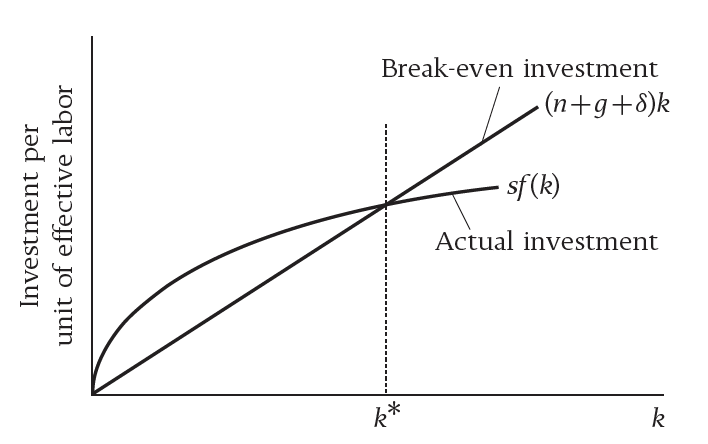
\includegraphics[width=0.6\linewidth]{figures/3_1.png}
				\caption{Dynamic Transition of Capital Per Unit of Effective Labor}
			\end{figure}
			
			\begin{figure}[h]
				\centering
				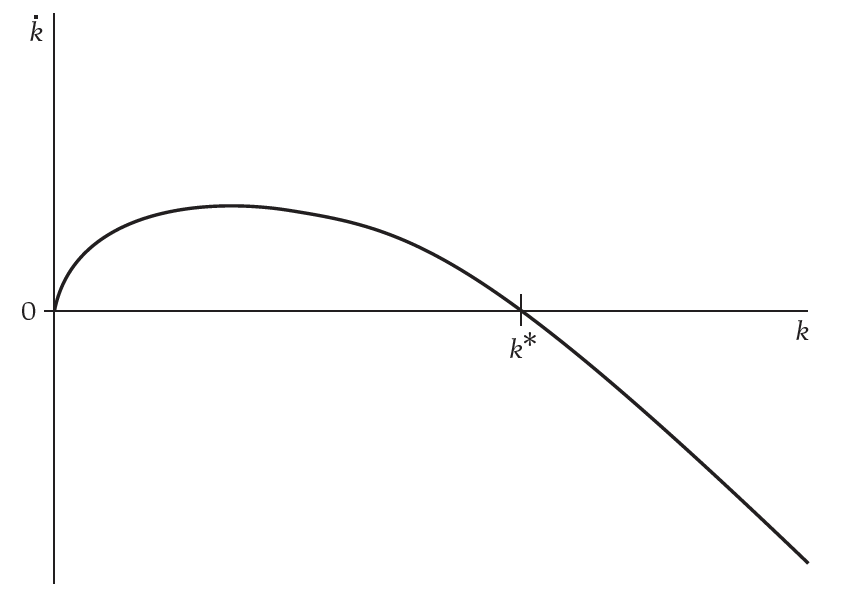
\includegraphics[width=0.6\linewidth]{figures/3_2.png}
				\caption{Phase Diagram of Capital Per Unit of Effective Labor}
			\end{figure}
			
			\newpage 
			
			\begin{definition}
			\textbf{Steady level of capital per unit of effective labor($k^*$)} is defined as the level of capital per unit of effective labor that equates break-even investment per unit of effective labor and actual investment per unit of effective labor. So that $k$ does not deviate from $k^*$.\footnote{The definition can also be expressed as $k^* := \{k \in \R_{\geq 0}: \dot{k}(k) = 0\}$}
				\begin{equation}
					k^* := \{k \in \R_{\geq 0}: sf(k) = (n+g+\delta) k\}
				\end{equation}
			\end{definition}
			\begin{remark}
				$k^* = 0$ is a trivial steady state.
			\end{remark}
			
			\begin{remark}
				The values of other endogenous variables at steady state are derived from $k^*$.
				\begin{example} Find the steady state growth rate of investment, consumption and output per unit of effective labor:
					\begin{gather}
						y^* = f(k^*) \\
						i^* = sf(k^*) = (n+g+\delta) k^* \\
						c^* = y^* - i^* = f(k^*) - (n+g+\delta)k^* = (1-s)f(k^*)
					\end{gather}
				\end{example}
				For the growth rate of each endogenous variable (per unit of effective labor). 
					\begin{gather}
						\pd{i(t)}{t}|_{k=k^*} = 0 \\
						\pd{c(t)}{t}|_{k=k^*} = 0 \\
						\pd{y(t)}{t}|_{k=k^*} = 0 
					\end{gather}
					above relations are equivalent to 
					\begin{gather}
						\tx{On steady state} \begin{cases}
							\dot{i}(t) = 0 \\
							\dot{c}(t) = 0 \\
							\dot{y}(t) = 0 \\
						\end{cases}
					\end{gather}
			\end{remark}
			
			\begin{proof}
				By definition of consumption per unit of effective labor,\\
				$c(\cdot) = (1-s)f(k(t))$ \\
				$\implies \dot{c}(t) := \pd{c(\cdot)}{t} = (1-s)f'(k(t)) \dot{k(t)}$ by chain rule \\
				Since $\dot{k}|_{k=k^*} = 0$ and $(1-s)f'(k(t)) < \infty$ \\
				Thus $\dot{c}(t)|_{k=k^*} = 0$ \\
				And $i(t) = sf(k(t))$, which is constant at $sf(k^*)$ at steady state. \\
			\end{proof}
			
		\subsection{Balanced Growth Path}
			\begin{definition}
				A \textbf{balanced growth path} is a situation where each variable in the model are all growing at a constant rate. \footnote{Variables are not required to grow at the same rate by this definition.} \footnote{Variables remaining fixed are also considered as growing at a constant rate ($g=0$).}
			\end{definition}
			
			\subsubsection{Growth Rates on Balanced Growth Path}
			\paragraph{Population and Technology} By definition of population and technological progress,
			\begin{gather}
				g_A := \frac{\dot{A}}{A} = g \\
				g_L := \frac{\dot{L}}{L} = n
			\end{gather}
			
			\paragraph{Capital per person} Since $\frac{K(t)}{L(t)} = \frac{k(t)A(t)L(t)}{L(t)} = k(t)A(t)$, and the growth rate of $x(t)$ can be found as $\pd{\ln{x(t)}}{t}$. Then
			\begin{proof}[Solution]
				\begin{gather}
					\pd{\ln{\frac{K(t)}{L(t)}}}{t} = \pd{k(t)A(t)}{t} \\
					= \pd{\ln{k(t)}}{t} + \pd{\ln{A(t)}}{t} \\
					= \frac{\dot{k}(t)}{k(t)} + g \\
				\end{gather}
				And at the steady state, by definition, $\dot{k}(t)|_{k=k^*} = 0$, therefore 
				\begin{equation}
					\textcolor{blue}{
						g_{\frac{K}{L}}^* = g
					}
				\end{equation}
			\end{proof}
			
			\paragraph{Output and Consumption per person} Similarly,
			\begin{proof}[Solution]
				\begin{gather}
					\frac{Y(t)}{L(t)} = y(t)A(t) \\
					g_{\frac{Y}{L}} = \pd{\ln{y(t)} + \ln{A(t)}}{t} \\
					= \pd{\ln{y}}{t} + \pd{\ln{A(t)}}{t} \\
					= g + \frac{\dot{y}}{y}
				\end{gather}
				and for consumption per person,
				\begin{gather}
					\frac{C(t)}{L(t)} = c(t)A(t)\\
					g_{\frac{C}{L}} = g + \frac{\dot{c}}{c} \\
				\end{gather}
				Thus, on the balanced growth path, \footnote{$g_X^*$ denotes the growth rate of variable $X$ on the balanced growth path.}
				\begin{gather}
					\textcolor{blue}{
						g_{\frac{Y}{L}}^* = g
					}
					\\
					\textcolor{blue}{
						g_{\frac{C}{L}}^* = g
					}
				\end{gather}
			\end{proof}
			
			\begin{proposition}
				Along the balanced growth path, consumption and output per person also grow at rate $g$.
			\end{proposition}
			
			\begin{proposition}
				Along the balanced growth path, aggregate variables, $Y(t), I(t), C(t)$ are all growing at a rate $n + g$.
				\begin{equation}
					\textcolor{blue}{
						g_{Y}^* = g_{C}^* = g_{I}^* = n + g
						}
				\end{equation}
			\end{proposition}
			\begin{proof}
				\begin{gather}
				g_{K} = \pd{\ln{K(t)}}{t} \\
				= \pd{\ln{A(t)L(t)k(t)}}{t} \\
				= \pd{\ln{A(t)}}{t} + \pd{\ln{L(t)}}{t} + \pd{\ln{k(t)}}{t} \\
				= g + n + \frac{\dot{k}}{k}
				\end{gather}
				and at balanced growth path, $\frac{\dot{k}}{k}|_{k=k^*} = 0$, therefore 
				\begin{equation}
					\textcolor{blue}{
						g_K^* = n + g
					}
				\end{equation}
				and proof for $C(t)$ and $I(t)$ are similar. \hl{Take log first, then separate the log and take derivative with respect to $t$.}
			\end{proof}
		
		\begin{definition}
			The \textbf{golden rule level of capital per unit of effective labor} ($k_G$) is the \ul{steady state level of} capital per unit of effective labor that maximizes steady state consumption per unit of effective labor.
				\begin{equation}
				\textcolor{red}{
					k_G = argmax_{k^* \in \textbf{k}^*(\Theta)} \{c^* = f(k^*) - (n+g+ \delta) k^*\}
					}
				\end{equation}
		\end{definition}
		
		\begin{definition}
			The \textbf{golden rule level of saving rate} $s_G$ is the saving rate such that the golden role level of capital per unit of effective labor is achieved.
		\end{definition}
		
		\begin{proof}[Proof. (First Order Necessary Condition for $k_G$)]
			\begin{gather}
				\pd{c^*(k^*)}{k^*} = 0 \\
				\implies \pd{f(k^*) - (n+g+\delta)k^*}{k^*} = 0 \\
				\implies f'(k^*) = (n+g+\delta)
			\end{gather}
			Thus, golden rule level of capital stock per unit of effective labor $k_G$ can be expressed as \footnote{Notice that the zero solution, $k^* = 0$ is a trivial steady state and we ignore this case during this course.}
			\begin{equation}
			\textcolor{red}{
				k_G = \{k \in \R_{+}: f'(k) = (n+g+\delta)\}
			}
			\end{equation}
		\end{proof}
		
		\subsection{Experiment}
			\subsubsection{Impact of Change in the Saving Rate ($s_1 > s_0$)}
			\par Suppose at time $t_0$, the saving rate parameter increases discretely: $s_0 \rightarrow s_1$.
			\begin{figure}[H]
				\centering
				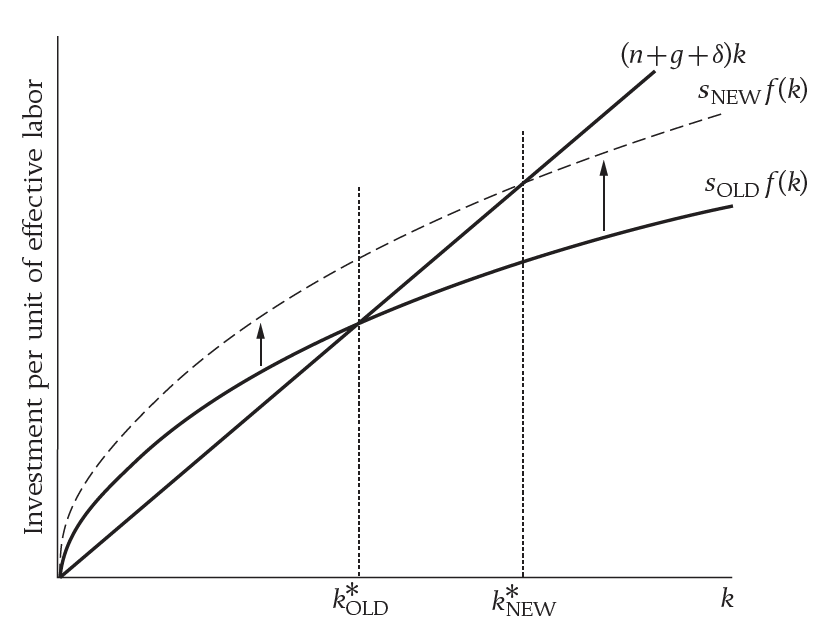
\includegraphics[width=0.5\linewidth]{figures/3_3.png}
				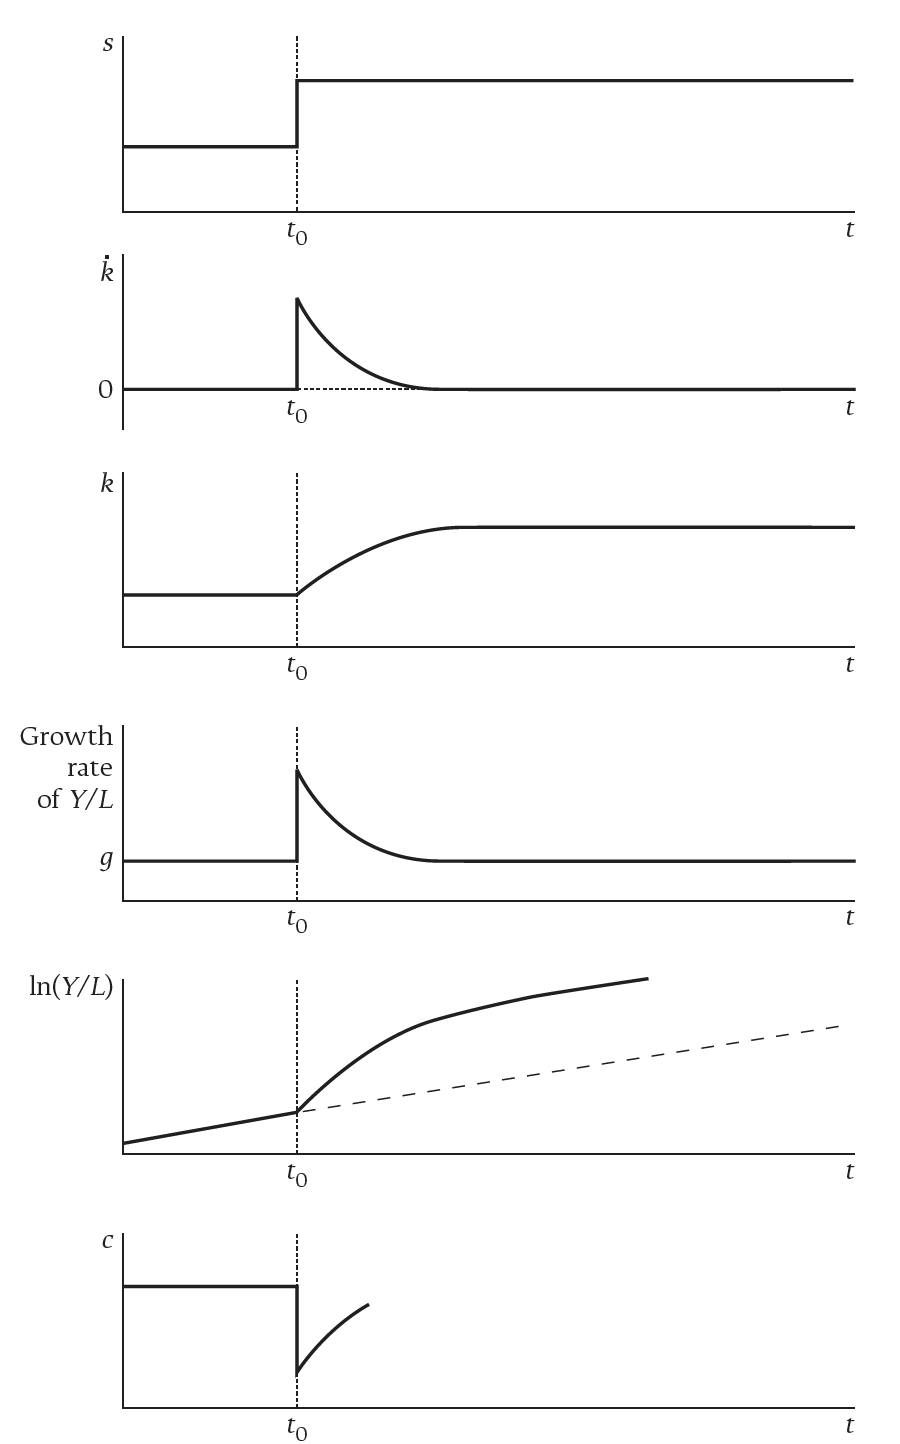
\includegraphics[width=0.5\linewidth]{figures/3_4.png}
				\caption{Effect of an Increase in Saving Rate.}
			\end{figure}
			
			\begin{remark}
				The relation of $c_0^*$ and $c_1^*$ depends on the relative position of $s_1$ and the golden rule level of saving rate $s_G$.
			\end{remark}
			
			\subsubsection{Derive the Effect of Change in $s$ Mathematically}
				\paragraph{Goal} Find $\pd{k^*}{s}$. And notice that $k^*(n+g+\delta) = sf(k^*)$ for any steady state capital level $k^*$. And the steady state level of capital per unit of effective labor can be written as a function of parameters, as $k^*(n, g, \delta, s)$.
				
			\paragraph{Impact on $k^*$}
			\begin{proof}[Solution]
				At any steady state level, $k^*$ satisfies \\
				\begin{equation}
					sf(k^*(n,g,\delta,s)) = (n+g+\delta)k^*(n,g,\delta,s)
				\end{equation}
				Differentiate both sides with respect to $s$, \\
				We have 
				\begin{equation}
					sf'(k^*)\textcolor{blue}{\pd{k^*}{s}} + f(k^*) = (n+g+\delta)\textcolor{blue}{\pd{k^*}{s}}
				\end{equation}
				Rearrange and get 
				\begin{equation}
					\pd{k^*}{s} = \frac{f(k^*)}{(n+g+\delta) - sf'(k^*)}
				\end{equation}
				Notice that the slope of break-even investment is greater than the slope of the actual investment at the steady state, therefore 
				\begin{equation}
					\pd{k^*}{s} > 0
				\end{equation}
			\end{proof}
			
			\paragraph{Impact on $y^*$}
			\begin{proof}[Solution]
				Using chain rule we have
				\begin{gather}
					\pd{y^*}{s} = \pd{f(k^*)}{s} \\
					= \pd{f(k^*)}{k^*} \pd{k^*}{s} > 0,\ \forall k^* \in \textbf{k}^*({\Theta})
				\end{gather}
			\end{proof}
			
			\par To get a sense on how much $y^*$ changes wit respect to change in $s$, we could look at the \ul{elasticity}.
			\begin{equation}
				\eta \equiv \pd{y^*}{s}\frac{s}{y^*} = f'(k^*) \pd{k^*}{s} \frac{s}{f(k^*)} = \frac{f'(k^*)s}{(n+g+\delta) - sf'(k^*)}
			\end{equation}
			Recall that $(n+g+\delta) = \frac{sf(k^*)}{k^*}$ and rearrange the elasticity
			\begin{gather}
				\eta = \pd{y^*}{s}\frac{s}{y^*} \\
				= \frac{f'(k^*)s}{(n+g+\delta) - sf'(k^*)} \\
				= \frac{s f'(k^*)}{\textcolor{blue}{\frac{s f(k^*)}{k^*}} - sf'(k^*)} \\
				= \frac{f'(k^*)}{\frac{f(k^*)}{k^*} - f'(k^*)} \\
				= \frac{f'(k^*) \frac{k^*}{f(k^*)}}{1 - f'(k^*)\frac{k^*}{f(k^*)}} \\
				= \textcolor{red}{
					\frac{\alpha_K}{1 - \alpha_K}
					}
			\end{gather}
			
			\begin{remark}
				$\alpha_K$ denotes the \ul{elasticity of output per unit of effective unit labor with respect to capital stock per unit of effective labor}, along the balanced growth path. And
				\[
					\alpha_K \approx \frac{1}{3}
				\]
			\end{remark}
			
			\begin{remark}
				If the production function is in the Cobb-Douglas form, then $\alpha_K = \alpha$.
			\end{remark}
			
			\begin{example}
				If $\alpha_K \approx \frac{1}{3}$ then \[\eta = \pd{y^*}{s} \frac{s}{y^*} \approx \frac{1}{2}\]
			\end{example}
			
			\paragraph{Impact on $c^*$} Notice that on the balanced growth path $c^* = y^* - i^*$.
			\begin{equation}
				c^* = f(k^*) - (n+g+\delta)k^*
			\end{equation}
			and differentiate with respect to $s$
			\begin{equation}
				\pd{c^*}{s} = [f'(k^*) - (n+g+\delta)] \pd{k^*}{s}
			\end{equation}
			And notice that the sign of $\pd{c^*}{s}$ depends on the relative slope of production function and break-even investment.
			By the first order condition of golden rule level of capital per unit of effective labor, $(n+g+\delta) = f'(k_G)$
			\begin{gather}
				\pd{c^*}{s} = [\textcolor{red}{f'(k^*) - f'(k_G)}]\pd{k^*}{s}
			\end{gather}
			And 
			\begin{equation*}
				\begin{cases}
					k^* = k_G \implies f'(k^*) = f'(k_G) \implies \pd{c^*}{s} = 0 \\
					k^* < k_G \implies f'(k^*) > f'(k_G) \implies \pd{c^*}{s} > 0 \\
					k^* > k_G \implies f'(k^*) < f'(k_G) \implies \pd{c^*}{s} < 0
				\end{cases}
			\end{equation*}
		\paragraph{Interpretation} when saving rate is less than the golden rule saving rate, increasing $s$ would lead to a higher steady state consumption, ($c^*$). \\
		when saving rate is higher than the golden rule level, increase saving rate would lead to a lower level of $c^*$.
	\section{Lecture 4 September 27. 2018}
	\subsection{Speed of Convergence}
	    \paragraph{Methodology} Look at the change in $k$ and linearize using first order Taylor's expansion.
	    \paragraph{Recall} $\dot{k}(t)$ is a function of $k(t)$ since 
	    \begin{equation}
	        \dot{k}(t) = sf(k(t)) - (n+g+\delta)k(t)
	    \end{equation}
	    And the first order Taylor series approximation of a function $f(x)$ around the point $x = x_0$.
	    \[
	        f(x) \approx f(x_0) + f'(x_0)(x - x_0)
	    \]
	    Then
	    \begin{gather}
	        \dot{k}(k) \approx \dot{k}(k^*) + \pd{\dot{k}(k)}{k}|_{k=k^*} (k - k^*) \\
	        = 0 + \pd{\dot{k}(k)}{k}|_{k=k^*} (k - k^*)
	    \end{gather}
	    Differentiating the both sides of equation (1) with respect to $k$.
	    \begin{gather}
	        \pd{\dot{k}(k)}{k}|_{k=k^*} = sf'(k^*) - (n + g + \delta) \\
	        = \frac{(n + g + \delta) k^*}{f(k^*)} f'(k^*) - (n + g + \delta) \\
	        = (n + g + \delta) \Big [
	            \frac{f'(k^*) k^*}{f(k^*)} - 1
	            \Big ] \\
	        = (n + g + \delta) (\alpha (k^*) - 1)
	    \end{gather}
	    where 
	    \begin{equation}
	    \textcolor{blue}{
	        \alpha_k (k^*) = f'(k^*)\frac{k^*}{f(k^*)}
	        }
	    \end{equation}
	    denotes the \ul{elasticity of $y$ with respect to $k$ \emph{at steady state}.}
	    
	    \subsubsection{Convergence of $k$}
	    \begin{gather}
	        \dot{k}(k(t)) \approx (n + g + \delta) (\alpha (k^*) - 1) (k(t) - k^*) \\
	        \implies \pd{({k - k^*}(k))}{t} = \dot{k}(k(t)) \approx (n + g + \delta) (\alpha (k^*) - 1) (k(t) - k^*)
	    \end{gather}
	    Let 
	    \begin{equation}
	    		\textcolor{red}{
	    		\lambda \equiv (n + g + \delta) (1 - \alpha (k^*))
	    		}
	    \end{equation}
		then 
	    \begin{gather}
	    \textcolor{orange}{
	        k(t) - k^* \approx e^{-\lambda t}(k(0) - k^*)
	    }
	    \end{gather}
	    \begin{remark}
		    \begin{proof}[Derive] (above equation)\\
		        Let $X(t) := k(t) - k^*$ \\
		        And since $\pd{k(t)}{t} = \pd{(k(t) - k^*)}{t}$ \\
		        Therefore $\dot{X}(t) = \dot{k}(t) \approx -\lambda X(t)$ \\
		        $\implies X(t) \approx X(0) e^{-\lambda t}$ \\
		        $\iff k(t) - k^* \approx (k(0) - k^*) e^{-\lambda t}$
		    \end{proof}
	    \end{remark}
	    \subsubsection{Convergence of $y$}
	    \begin{gather}
	        y(t) = f(k(t)) \\
	        \implies \dot{y}(t) = f'(k(t))\dot{k}(t) \\
	        \tx{(Take the first order Taylor series approximation around $k=k^*$)} \\
	        \implies y(t) \approx f(k^*) + f'(k^*) (k(t)-k^*) \\
	        \implies y(t) - y^* \approx f'(k^*)(k(t) - k^*) \\
	        \implies \frac{\dot{y}(t)}{y(t) - y^*} = \frac{f'(k^*)\dot{k}(t)}{f'(k^*)(k(t) - k^*)} = \frac{\dot{k}(t)}{k(t) - k^*} \approx - \lambda \\
	       \implies \textcolor{orange}{
	       		y(t) - y^* \approx e^{- \lambda t} (y(0) - y^*)
	       }
	    \end{gather}
	    
	    \begin{example}
	        How long does it take to move 1/2 way to the balance growth path. Assuming population growth rate is $2\%$, growth in output per worker is $2\%$ and depreciation is $2\%$ and  $\alpha_K = \frac{1}{3}$.
	        \begin{proof}[Solution]
	            $\lambda = (1 - \alpha_K)(n + g + \delta)$ 
	            Since we know along the balanced growth path, \begin{gather}
	                \frac{Y(t)}{L(t)} = y^* A(t) \\
	                \implies \pd{\ln{\frac{Y(t)}{L(t)}}}{t} = g
	            \end{gather}
	            Therefore $g = 0.02$ and therefore $\lambda = 0.04$. \\
	            To find the date where we have moved half way we need to solve 
	            \begin{gather}
	                \frac{y(\tilde{t}) - y^*}{y(0) - y^*} = 0.5 \approx e^{-\lambda t}\\
	                \implies \ln(0.5) \approx -\lambda \tilde{t} \\
	                \implies \tilde{t} = \frac{-\ln(0.5)}{0.04} \approx 17.33
	            \end{gather}
	        \end{proof}
	    \end{example}
	    
	    \subsection{Implications}
	    \par Solow growth model identifies 2 sources of \ul{output per worker}:
	    \begin{equation}
		    	\frac{Y(t)}{L(t)} = \frac{F(K(t), A(t)L(t))}{L(t)} = F(\frac{K(t)}{L(t)}, A(t))
	    \end{equation}
	    \begin{enumerate}
	    	\item Differences in the among of \hl{capital per worker}, $\frac{K}{L}$.
	    	\item Differences in the \hl{effectiveness of productivity} of labor, $A$.
	    \end{enumerate}
	    Notice that in the long run balanced growth path
	    \begin{gather}
	    	\frac{K(t)}{L(t)} = k(t)A(t) \\
	    	\implies \pd{\ln(\frac{K(t)}{L(t)})}{t} = \frac{\dot{k}(t)}{k(t)} + \frac{\dot{A}(t)}{A(t)}
	    \end{gather}
	    Therefore along the balanced growth path $\dot{k}(t) = 0$ so only the growth in $A$ matters.
	    
	    \subsection{Growth Accounting}
	    \par Consider the growth rate of aggregate output $Y(t)$, taking the total derivatives gives
	    \begin{gather}
	    	\dot{Y}(t) = \pd{Y(t)}{K(t)} \pd{K(t)}{t} + \pd{Y(t)}{L(t)} \pd{L(t)}{t} + \pd{Y(t)}{A(t	)}\pd{A(t)}{t} \\
	    	\implies 
	    	\frac{\dot{Y}(t)}{Y(t)} = \pd{Y(t)}{K(t)} \frac{1}{Y(t)} \pd{K(t)}{t} + \pd{Y(t)}{L(t)} \frac{1}{Y(t)} \pd{L(t)}{t} + \pd{Y(t)}{A(t)} \frac{1}{Y(t)} \pd{A(t)}{t} 
	    \end{gather}
	    Then express the equation in terms of growth rates in $K, L, A$ variables,
	    \begin{gather}
	    	\frac{\dot{Y}(t)}{Y(t)} = \textcolor{orange}{\pd{Y(t)}{K(t)} \frac{K(t)}{Y(t)}}\frac{\pd{K(t)}{t}}{K(t)} 
	    	+ \textcolor{red}{\pd{Y(t)}{L(t)} \frac{L(t)}{Y(t)}} \frac{\pd{L(t)}{t}}{L(t)} 
	    	+ \textcolor{blue}{\pd{Y(t)}{A(t)} \frac{A(t)}{Y(t)} \frac{\pd{A(t)}{t}}{A(t)}}
	    	\\
	    	= \textcolor{orange}{\alpha_K} \frac{\dot{K}(t)}{K(t)} 
	    	+ \textcolor{red}{\alpha_L} \frac{\dot{L}(t)}{L(t)} 
	    	+ \textcolor{blue}{R(t)} \\
	    = \alpha_K \ g_K(t) + \alpha_L \ g_L(t) + R(t)
	    \end{gather}
	    where $R(t)$ is the \textbf{Solow Residual} and 
	    \begin{equation}
	    	\textcolor{red}{R(t) = \pd{Y(t)}{A(t)} \frac{A(t)}{Y(t)} \frac{\dot{A}(t)}{A(t)}}
	    \end{equation}
	    And $\alpha_K(t)$ and $\alpha_L(t)$ denote the elasticity of output with respect to capital and labor respectively.
	    
	    \begin{example}
	    	Assume the output growth is $40\%$ and capital growth is $20\%$ and labor growth is $30\%$. If $\alpha_K = 0.3$ and $\alpha_L = 0.7$. What's the contribution to output growth of capital?
	    	\[
	    		\alpha_K \frac{\dot{K}(t)}{K(t)} = 0.3 \times 20\% = 0.06
	    	\]
	    	and the contribution from labor is
	    	\[
	    		\alpha_L \frac{\dot{L}(t)}{L(t)} = 0.7 \times 30\% = 0.21
	    	\]
	    	and the Solow residual is 
	    	\[
	    		R(t) = g_Y - 6\% - 21\% = 0.4 - 0.06 - 0.21 = 0.13
	    	\]
	    \end{example}
	    
	    \begin{example}
	    	Let's assume the economy is on its balanced growth path. Assume that a change in medicine increase survival rate during child birth. \\
	    	What would the effect of this be on steady state $k^*, y^*, c^*, i^*$.\\
	    	First show the growth that despite break-even investment and actual investment. Label the steady state values. \\
	    \end{example}
	    
	    \begin{proof}[Solution]
	    	\textbf{The effect would be an increase in $n$} \\
	    	Suppose $n_0 \to n_1$ with $n_0 < n_1$. \\
	    	Therefore $k^*$ falls, and $y^*$ falls. \\
	    	Since consumption and actual investment are constant frictions of $y^*$, \\
	    	Therefore both $c^*, i^*$ falls.
	    	\begin{figure*}[h]
	    		\centering
	    		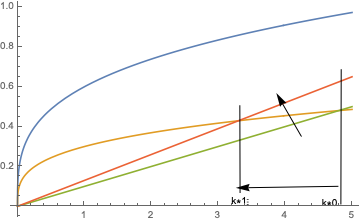
\includegraphics[width=0.7\linewidth]{figures/4_1}
	    	\end{figure*}
	    \end{proof}
	
	\section{Lecture 5 October 11. 2018}
	\subsection{Economy Setup}
	\begin{itemize}
		\item Infinite horizon continuous time model.
		\item Exogenous growth rates of technology/productivity and population.
		\begin{gather}
			\textcolor{orange}{A(t) = A(0) e^{gt}} \\
			\textcolor{orange}{L(t) = L(0) e^{nt}}
		\end{gather}
		
		\item (\ul{Endogenous saving decisions}) A key difference of endogenous growth model from the Solow model is that the saving decision and the capital stock are determined by the interaction of utility/profit maximizing households and firms.
	\end{itemize}
	
	\subsection{Households}
	\subsubsection{Assumptions and Behaviours}
	\begin{assumption}(Setup)
		\begin{itemize}
			\item There are a large numbers of \ul{identical} households in the economy ($H$). \emph{To ensure that \ul{no household has market power}.}
			\item And the size of each household are assumed to grow at rate $n$.
			\item Each household has $\frac{L(t)}{H}$ members in it at time $t$.
			\item Each household has \emph{initial} capital holding of $\frac{K(0)}{H}$.
			\item Each member of the household supplies 1 unit of labor at each point in time \ul{inelastically}. (\emph{No uncertainty})
			\item For simplicity, there's no depreciation of capital stock. ($\delta = 0$)
			\item Capital is rented to firms at rate $r(t)$. (Note that households invest in the form of capital accumulation)
			\item Labor is hired at wage rate $W(t) = w(t)A(t)$. Where $W(t)$ is the wage per unit of labor and $w(t)$ is the wage per unit of effective labor.
		\end{itemize}
	\end{assumption}
	
	\begin{remark}[Implicit Assumption]
		Firms are owned by households and rebate all profits earned (if any) back to households. But since markets are assumed to be competitive, altogether with the assumption of constant return to scale, firms are earning no profit.
	\end{remark}
	
	\subsubsection{Objective Functions}
	\par Household's \emph{objective function} is given by the \textbf{Lifetime Utility Function}
	\begin{equation}
		\textcolor{orange}{
			U = \int_{t=0}^\infty {e^{-\rho t} u(C(t)) \frac{L(t)}{H}}\ dt,\ \rho > 0
		}
	\end{equation}
	where $\rho$ is the \textbf{discount rate} and $C(t)$ is the \textbf{consumption \ul{per person}}.
	\begin{remark}
		$\rho$ measures \ul{consumers' attitude between present and future utilities}.
		When $\rho = 0$, household values utility in the future equally. 
		When $\rho > 0$, household values future utility less than present utility.
		The greater $\rho$ is, the less value household puts on future consumption/utility (\emph{i.e. consumers are less patient}).
		Notice that $\rho$ cannot be negative in this model, since with $\rho < 0$ household values utility at $t=\infty$ infinitely more than current utility, the lifetime utility does not converge. For instance, with $\rho < 0$, $e^{-\rho t}$ is increasing in $t$, then infinite-horizon household could attain infinite utility by allocating consumption at $t=\infty$.
		\footnote{Intuitively, if $\rho < 0$, households could save everything and spend their saving when $t > \infty$. This scenario is certainly unrealistic.}
	\end{remark}
	
	\subsubsection{Household Budget Constraints}
	\par Household's budget is given in terms of \ul{present discounted value}. \\
	Since the household has $\frac{L(t)}{H}$ members, labor income at time $t$ is 
	\begin{equation}
		A(t)w(t)\frac{L(t)}{H} = W(t)\frac{L(t)}{H}
	\end{equation}
	The amount of consumption for the household at the time $t$ is 
	\begin{equation}
		C(t)\frac{L(t)}{H}
	\end{equation}
	And let $R(t)$ denote the \textbf{continuously compounding interest rate} at time $t$:
	\begin{equation}
		R(t) := \int_{\tau=0}^t r(\tau)\ d\tau
	\end{equation}
	\begin{remark}
		We know under \ul{continuously compounding interest}, one unit of output invested at $\tau=0$ is worth $e^{R(t)}$ units at $\tau=t$. Conversely, 1 unit of output at $\tau=t$ is worth $e^{-R(t)}$ at $\tau=0$.
	\end{remark}
	\begin{remark}
		The budget constraint implies that the \ul{present discounted value of lifetime consumption} must not exceed the \ul{present discounted value of labor income} plus \ul{initial wealth/capital}.
	\end{remark}
	\par And the household lifetime budget constraint is given by
	\begin{equation}
		\textcolor{orange}{
			\int_{t=0}^\infty e^{-R(t)} C(t) \frac{L(t)}{H}\ dt \leq \frac{K(0)}{H} + \int_{t=0}^\infty e^{-R(t)} w(t) \frac{A(t)L(t)}{H}\ dt
		}
	\end{equation}
	\\
	Then normalize budget constraint (5) into \emph{per unit of effective labor variables} to get an equivalent form.
	\begin{gather}
		\int_{t=0}^\infty e^{-R(t)} C(t) \frac{L(t)}{H}\ dt  \leq \frac{K(0)}{H} + \int_{t=0}^\infty e^{-R(t)} w(t) \frac{A(t)L(t)}{H}\ dt \\
		\iff 
		\int_{t=0}^\infty e^{-R(t)} c(t) \frac{A(t)L(t)}{H}\ dt \leq \frac{k(0)A(0)L(0)}{H} + \int_{t=0}^\infty e^{-R(t)} w(t) \frac{A(t)L(t)}{H}\ dt \\ 
		\iff \int_{t=0}^\infty e^{-R(t)} c(t) e^{(n+g)t} \frac{A(0)L(0)}{H}\ dt \leq \frac{k(0)A(0)L(0)}{H} + \int_{t=0}^\infty e^{-R(t)} w(t) e^{(n+g)t}\frac{A(0)L(0)}{H}\ dt \\
		\iff \textcolor{red}{\int_{t=0}^\infty e^{-R(t)} e^{(n+g)t} c(t)\ dt \leq k(0) + \int_{t=0}^\infty e^{-R(t)} e^{(n+g)t} w(t)\ dt}
	\end{gather}
	The \textbf{assets} owned by household on date $s$, $\frac{K(s)}{H}$, is given by \emph{reverse discounting saving and initial capital to $\tau=s$}.
	\begin{gather}
		\frac{K(s)}{H} = e^{R(s)} \frac{K(0)}{H} + \int_{t=0}^s e^{-R(t)+R(s)} \Big\{\frac{w(t)A(t)L(t)}{H} - \frac{c(t)A(t)L(t)}{H} \Big\}\ dt \\
		= e^{R(s)} \frac{K(0)}{H} +  \int_{t=0}^s e^{-R(t)+R(s)} \{w(t) - c(t)\} \frac{A(t)L(t)}{H} dt \\
		\implies \textcolor{blue}{
		e^{-R(s)} \frac{K(s)}{H} \equiv \frac{K(0)}{H} + \int_{t=0}^s e^{-R(t)} \{w(t) - c(t)\} \frac{A(t)L(t)}{H}\ dt}
	\end{gather}
	Substitute to the budget constraint,
	\begin{gather}
		\frac{K(0)}{H} + \int_{t=0}^\infty e^{-R(t)} \frac{w(t)A(t)L(t)}{H}\ dt - \int_{t=0}^\infty e^{-R(t)} \frac{c(t)A(t)L(t)}{H}\ dt \geq 0 \\
		\iff \frac{K(0)}{H} + \int_{t=0}^\infty e^{-R(t)} \{w(t) - c(t)\} \frac{A(t)L(t)}{H}\ dt \geq 0 \\
		\iff \lim_{s \to \infty}\Big\{ \frac{K(0)}{H} + \int_{t=0}^s e^{-R(t)} \{w(t) - c(t)\} \frac{A(t)L(t)}{H}\ dt \Big \} \geq 0 
	\end{gather}
	\begin{equation}
		\textcolor{blue}{
			\implies \lim_{s\to \infty}e^{-R(s)}\frac{K(s)}{H} \geq 0
		}
	\end{equation}
	These implies that the household's asset holding cannot be negative at the limit. And this is a \textbf{no-Ponzi game} condition.
	
	\begin{proposition}
		The integral form budget constraint and non-Ponzi game condition is equivalent.
	\end{proposition}
	
	\begin{definition}
		A \textbf{Ponzi game} is a scheme in which someone issues debt and rolls it over forever. In other words, the person always pays off debt by issuing more debt.
	\end{definition}
	
	\begin{remark}
		If households could run a Ponzi scheme, then the present value of lifetime consumption can exceed the present value of lifetime resources.
	\end{remark}
	
	\subsection{Instantaneous Utility Function}
	
	\begin{definition}[Coefficient of Relative Risk Aversion]
		Given an utility function $u(c): \R_{\geq 0} \to \R$, the coefficient of relative risk aversion of it is defined as
		\begin{equation}
			CRRA(u) \equiv - \frac{c u''(c)}{u'(c)}
		\end{equation}
	\end{definition}
	
	\begin{assumption}
		The household \textbf{instantaneous utility function} is assumed to be in the form of constant relative risk aversion (CRRA) as 
		\begin{equation}
		\textcolor{orange}{
			u(C(t)) = \frac{C(t)^{1 - \theta}}{1 - \theta}
			}
		\end{equation}
	\end{assumption}
	And lifetime utility function becomes
	\begin{gather}
		U = \int_{t=0}^\infty e^{-\rho t} \frac{(A(t)c(t))^{1-\theta}}{1-\theta} e^{nt} \frac{L(0)}{H}\ dt\\
		\int_{t=0}^\infty e^{-\rho t} \frac{c(t)^{1-\theta}}{1-\theta} A(0)^{1-\theta} e^{(1-\theta)gt} e^{nt} \frac{L(0)}{H}\ dt\\
		= A(0)^{1 - \theta} \frac{L(0)}{H} \int_{t=0}^\infty {e^{-\rho t + nt + (1-\theta)gt} \frac{c(t)^{1-\theta}}{1-\theta}\ dt} \\
		= A(0)^{1 - \theta} \frac{L(0)}{H} \int_{t=0}^\infty {e^{-(\rho - n - (1-\theta)g)t} \frac{c(t)^{1-\theta}}{1-\theta}\ dt}
	\end{gather}
	\begin{equation}
	\textcolor{orange}{
		B \int_{t=0}^\infty e^{-\beta t}\frac{c(t)^{1-\theta}}{1- \theta}\ dt
	}
	\end{equation}
	where
	\begin{equation}
		B := A(0)^{1-\theta} \frac{L(0)}{H}\tx{ and } \beta := \rho - n - (1-\theta)g
	\end{equation}
	\begin{assumption}
		Assuming $\theta > 0$ and $\beta = \rho - n - (1-\theta)g > 0$.
	\end{assumption}
	
	\begin{remark}
		If $\beta \leq 0$ then the integral would diverge and the maximization problem does not have a well-defined solution.
	\end{remark}
	
	\section{Lecture 6 Oct 18. 2018}
		\subsection{Firm Setup}
			\begin{assumption}
				Firms 
				\begin{itemize}
					\item are all \emph{identical} and 
					\item employ stocks of capital and labor
					\item perfectly competitive in factor markets (no control over wage and rent)
					\item maximize profits
					\item each firm has access to the production function $Y = F(K, AL)$
				\end{itemize}
			\end{assumption}
			\begin{notation} Let
				\begin{itemize}
					\item $w(t)$ denote the \emph{real} wage per unit of effective labor
					\item $r(t)$ denote the rental rate of capital
					\item $A(t)$ denotes the labor augmenting technology/ knowledge
				\end{itemize}
			\end{notation}
			\begin{remark}
				The profit is given by 
				\begin{equation}
					\pi(t) = F(K(t), A(t)L(t)) - w(t)A(t)L(t) -r(t) K(t)
				\end{equation}
			\end{remark}
			\begin{assumption}
				Technology in this model, $A(t)$, is \ul{given exogenously} so it isn't a choice for firms.
			\end{assumption}
			
		\subsection{Firm's Optimization}
			\paragraph{Maximization} \footnote{Note since $A(t)$ is given exogenously, the arguments of maximization could also be written as $\max_{K(t), A(t)L(t)}$}
			\begin{gather}
				\max_{K(t), L(t)} \pi(t) = F(K(t), A(t)L(t)) - w(t)A(t)L(t) -r(t) K(t)
			\end{gather}
			
			\paragraph{First Order Condition}
			\begin{gather}
				K(t) : \pd{F(K(t), A(t)L(t))}{K(t)} - r(t) = 0 \\
				L(t) : \pd{F(K(t), A(t)L(t))}{L(t)} - w(t)A(t) = 0
			\end{gather}
			
			\begin{example}[Cobb-Douglas Form]
				Consider 
				\begin{equation}
					F(K(t), A(t)L(t)) = K^\alpha (AL)^{1-\alpha}
				\end{equation}
				Taking the first order necessary condition for profit maximization:
				\begin{gather}
					K(t) : \alpha K^{\alpha - 1} (AL)^{1-\alpha} = r(t)\\
					L(t) : (1-\alpha) K^\alpha (AL)^{-\alpha}A(t) =A(t) w(t)
				\end{gather}
				In per-effective-unit-of-labor form
				\begin{gather}
					\alpha k(t) ^ {\alpha - 1} = r(t) \\
					(1-\alpha) k(t) ^ \alpha = w(t) \\
				\end{gather}
			\end{example}
			In general we could have the following first order necessary conditions in terms of the per unit of effective labor variables.
			\begin{gather}
			\textcolor{blue}{
				f'(k(t)) = r(t)
			} \\
			\textcolor{blue}{
				f(k(t)) - k(t) f'(k(t)) = w(t)
			}
			\end{gather}
			
			\begin{proof}
    			\begin{gather}
    			    r(t) = \pd{F(\cdot)}{K} 
    			    = \pd{AL f(\frac{K}{AL})}{K} \\
    			    = AL \pd{f(k)}{k} \pd{\frac{K}{AL}}{K} 
    			    = \pd{f(k)}{k} 
    			    = f'(k)
    			\end{gather}
			\end{proof}
			
			\begin{proof}
                \begin{gather}
                    A(t)w(t) = \pd{F(K, AL)}{L} = \pd{AL f(\frac{K}{AL})}{L} \\
                    = Af(k) + AL \pd{f(\frac{K}{AL})}{AL} \pd{AL}{L} \\
                    = Af(k) + AL \pd{f(\frac{K}{AL})}{k} \pd{\frac{K}{AL}}{AL} \pd{AL}{L} \\
                    = Af(k) + A^2 L f'(k) \frac{-K}{(AL)^2} \\
                    = Af(k) - k f'(k) \frac{A^2 L}{AL} \\
                    = Af(k) - k f'(k) A \\
                    \implies w(t) = f(k) - k f'(k)
                \end{gather}
			\end{proof}
			
		\subsection{Household Behaviour}
			\par Household are going to chose a function $\mc{C}(t): [0, \infty) \to \R_{\geq 0}$, or equivalently, a set of consumption values, $\{c(t)\}_{t=0}^\infty$, to maximize lifetime utility subjected to their lifetime budget constraint.
			\begin{gather}
				\max_{\{c(t)\}_{t=0}^\infty} B \int_{t=0}^\infty e^{-\beta t} \frac{c(t)^{1-\theta}}{1-\theta}\ dt \\
				s.t.\ 0 \leq k(0) + \int_{t=0}^\infty {e^{-R(t)} e^{(n+g)t} (w(t) - c(t))\ dt}
			\end{gather}
			Setup Lagrangian at each time point,
			\begin{equation}
				\mc{L} = B \int_{t=0}^\infty e^{-\beta t} \frac{c(t)^{1-\theta}}{1-\theta}\ dt + \lambda \Big [ k(0) + \int_{t=0}^\infty {e^{-R(t)} e^{(n+g)t} (w(t) - c(t))\ dt} \Big ]
			\end{equation}
			\paragraph{First Order Necessary Conditions}
				On an arbitrary time period $t$,
				\begin{gather}
					c(t): B e^{-\beta t} c(t) ^{-\theta} - \lambda e^{-R(t)} e^{(n+g)t} = 0 \\
					\lambda: k(0) + \int_{t=0}^\infty {e^{-R(t)} e^{(n+g)t} (w(t) - c(t))\ dt} = 0
				\end{gather}
		\subsection{The Behaviour of Consumption}
			\par The the log of both size of (2) gives 
			\begin{gather}
				\ln(B) + \ln(e^{-\beta t}) + \ln(c(t)^{-\theta}) = \ln(\lambda) + \ln(e^{-R(t)}) + \ln(e^{(n+g)t}) \\
				\iff \ln(B) - \beta t - \theta \ln(c(t)) = \ln(\lambda) - R(t) + (n+g)t \\
				\tx{Since above equation holds for all $t$, take the derivative with respect to $t$} \\
				\implies -\beta - \theta \frac{\dot{c}(t)}{c(t)} = -r(t) + (n+g) \\
				\iff \frac{\dot{c}(t)}{c(t)} = \frac{r(t) - \beta - (n + g)}{\theta} \\
				\because \beta = \rho - n - (1-\theta) g\\
				\iff 
				\textcolor{red}{
					\frac{\dot{c}(t)}{c(t)} = \frac{r(t) - \rho - \theta g}{\theta}
				}
			\end{gather}
			
			\begin{remark}
				The growth rate of consumption \ul{per person} is given by
				\begin{equation}
					\pd{\ln(C(t))}{t} = \frac{r(t)-\rho}{\theta}
				\end{equation}
			\end{remark}
			\begin{remark}
				Go backwards by solving the ODE
				\begin{gather}
					\frac{\dot{c}(t)}{c(t)} = \frac{r(t) - \rho - \theta g}{\theta} = \pd{\ln(c(t))}{t} \\
					\implies c(t) = c(0) e^{\frac{R(t) - (\rho + \theta g)t}{\theta}}
				\end{gather}
				Using the budget constraint to solve for $c(0)$.
				\begin{gather}
					k(0) + \int_{t=0}^\infty {e^{-R(t)} e^{(n+g)t} w(t)\ dt} = \int_{t=0}^\infty {e^{-R(t)} e^{(n+g)t} c(t)\ dt} \\
					= \int_{t=0}^\infty {e^{-R(t)} e^{(n+g)t} c(0) e^{\frac{R(t) - (\rho + \theta g)t}{\theta}}}\ dt \\
					= c(0) \int_{t=0}^\infty e^{(\frac{1}{\theta} - 1)R(t)} e^{(n - \frac{\rho}{\theta})t} \ dt \\
					\implies
					\textcolor{red}{
					c(0) = \frac{
					k(0) + \int_{t=0}^\infty {e^{-R(t)} e^{(n+g)t} w(t)\ dt}
					}{
					\int_{t=0}^\infty e^{(\frac{1}{\theta} - 1)R(t)} e^{(n - \frac{\rho}{\theta})t} \ dt
					}
					}
				\end{gather}
			\end{remark}
		\subsection{Dynamics of the Economy}
		\subsubsection{Dynamic of $c$}
		\par From the firms problem, $r(t) = f'(k(t))$, so at equilibrium, 
		\begin{equation}
			\frac{\dot{c}(t)}{c(t)} = \frac{f'(k(t)) - \rho - \theta g}{\theta}
		\end{equation}
		In the long run, $\dot{c}(t) = 0$. This happens if and only if (note that we have $\delta=0$.)
		\begin{equation}
			f'(k^*) = \rho + \theta g
		\end{equation}
		Therefore 
		\begin{equation}
			\frac{\dot{c}(t)}{c(t)} = \frac{f'(k(t)) - f(k^*)}{\theta}
		\end{equation}
		That's, $k(t) < k^* \implies f'(k(t)) > f(k^*) \implies \dot{c}(t) > 0$.
		\begin{figure*}[h]
			\centering
			\caption{Phase diagram of $\dot{c}$ and $\dot{k}$}
			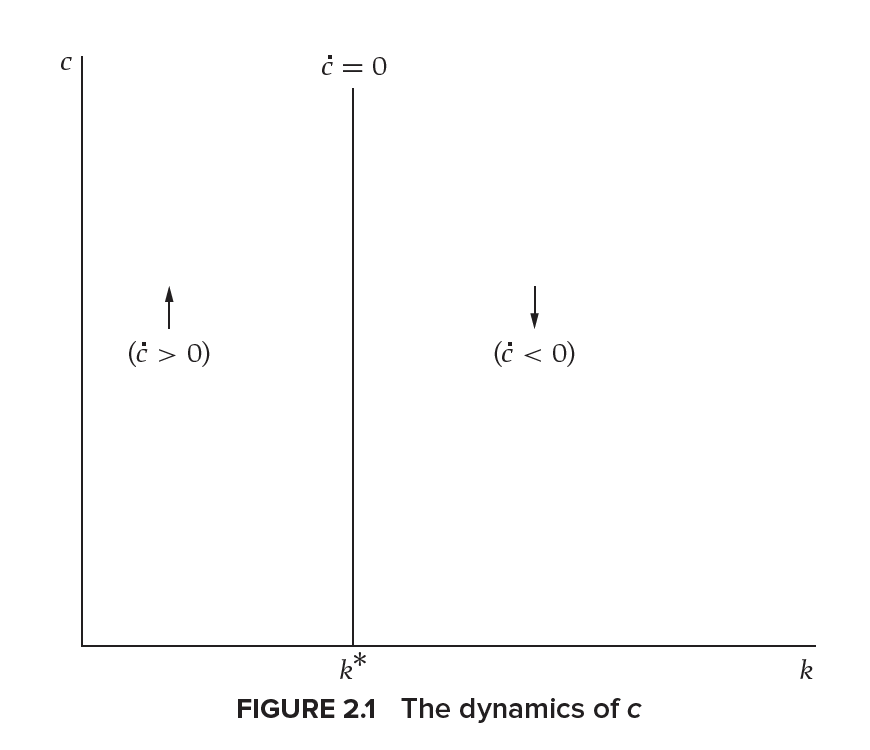
\includegraphics[width=0.45\linewidth]{figures/6_1}
			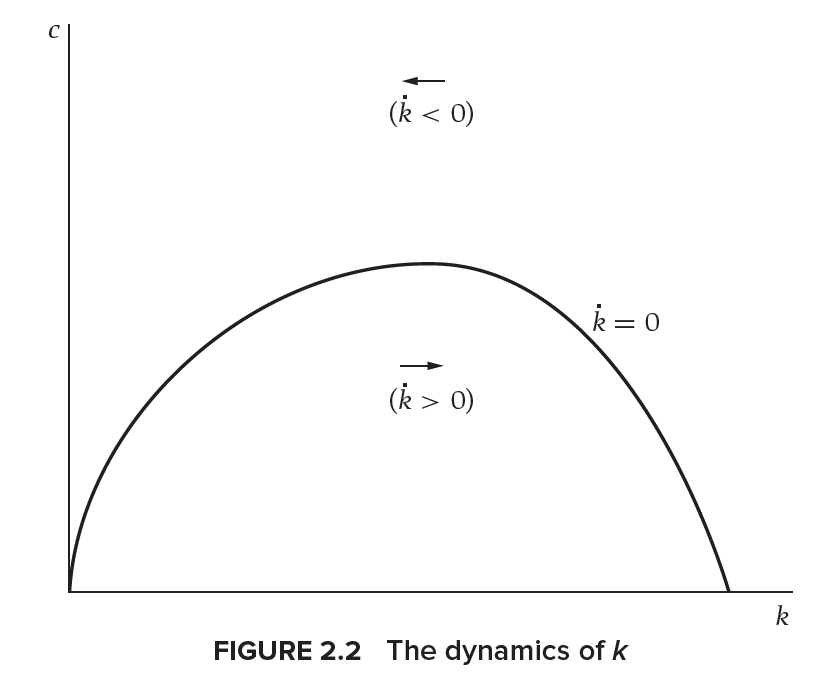
\includegraphics[width=0.45\linewidth]{figures/6_2}
		\end{figure*}
		
		\subsubsection{Dynamic of $k$}
		\par Assuming there's no depreciation ($\delta=0$)
		\begin{equation}
			\dot{k}(t) = f(k(t)) - c(t) - (n+g)k(t)
		\end{equation}
%		\begin{figure*}[h]
%			\centering
%			\caption{Phase diagram of $\dot{k}$}
%			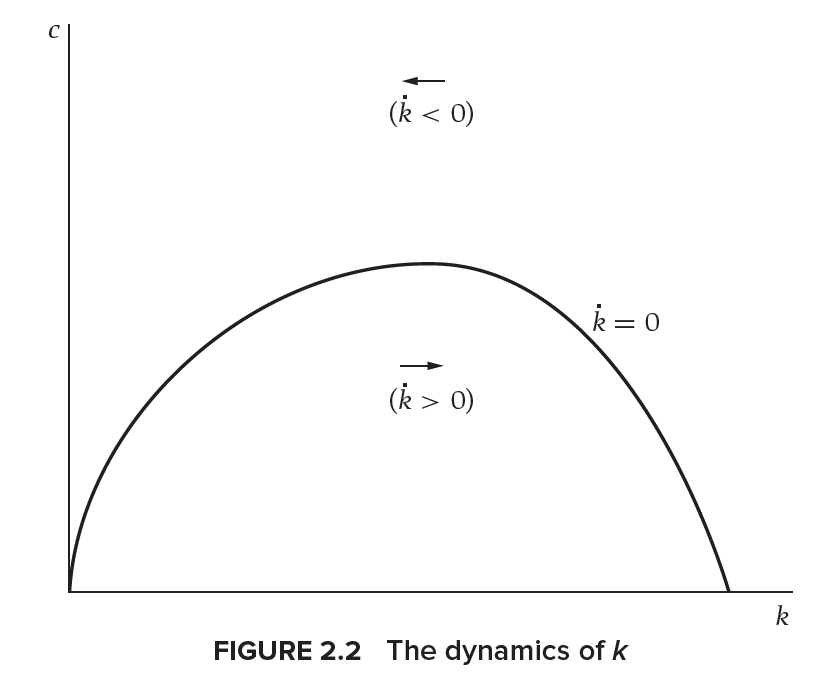
\includegraphics[width=0.6\linewidth]{figures/6_2}
%		\end{figure*}
		Below the $\dot{k} = 0$ curve, $\dot{k} > 0$ since actual investment per unit of effective labor exceeds the break-even level of investment per unit of effective labor.
		\\
		Putting two phase diagrams together,
		\begin{figure*}[h]
			\centering
			\caption{Combined phase diagram}
			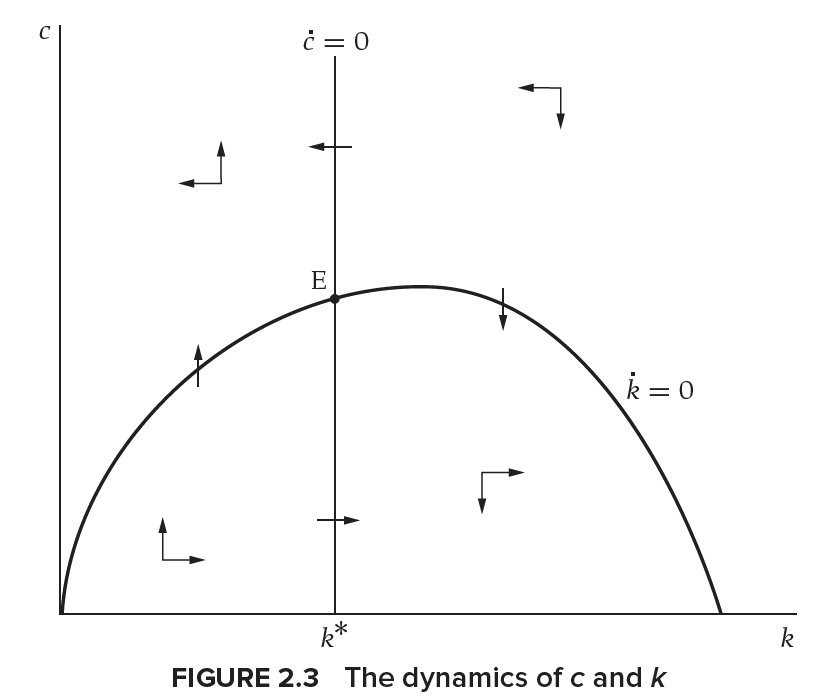
\includegraphics[width=0.5\linewidth]{figures/6_3}
		\end{figure*}
		The \textbf{steady state} is given at point $E$, where $\dot{c} = \dot{k} = 0$.
		
		\newpage
		\subsubsection{Initial Point Problem (Saddle Path)}
		\par For any given value of $k(0)$ and the budget constraint satisfied, there exists an \ul{unique} value of $c(0)$, so that one economy starts with $(k(0), c(0))$ would evolve and converge to the steady state $E$. Such path of convergence is called \textbf{saddle path}.
		\begin{figure*}[h]
			\centering
			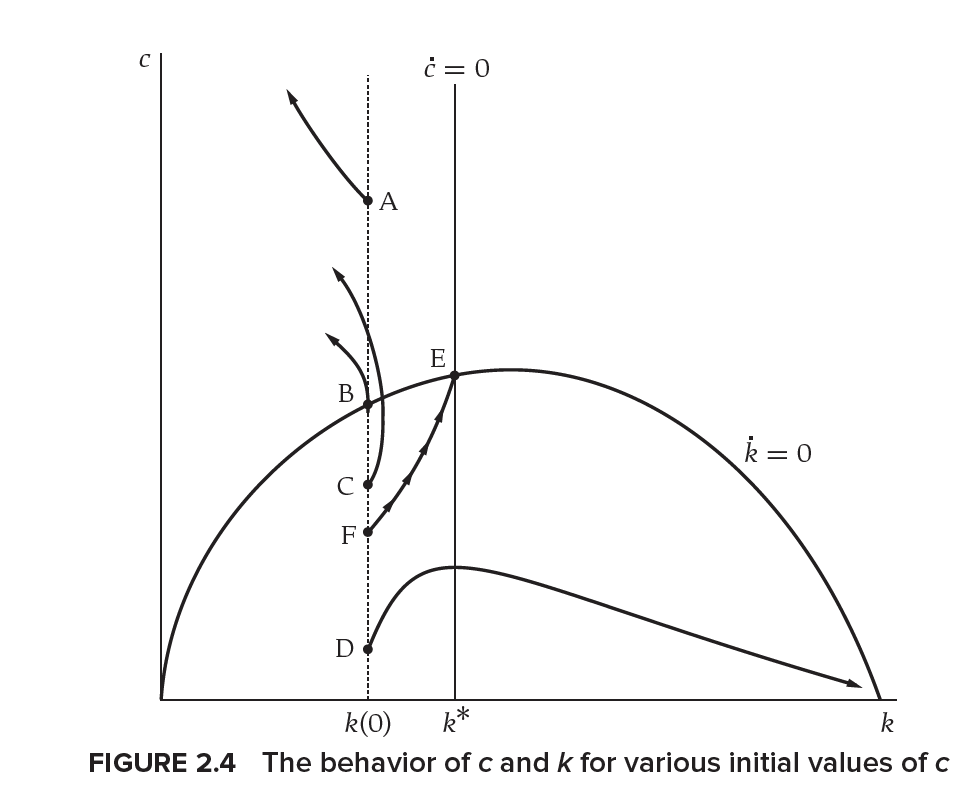
\includegraphics[width=0.5\linewidth]{figures/6_4}
		\end{figure*}


	\section{Lecture 7 Oct. 25 2018}
		\begin{remark}[Conditions on Phase Diagram] The phase diagram and saddle path are constructed from the following conditions,
			\begin{enumerate}
				\item Euler equation of $c$ \[ \frac{\dot{c}(t)}{c(t)} = \frac{f'(k(t)) - \rho - \theta g}{\theta} \]
				\item Dynamic transition of $k$ (state equation) \[ \dot{k}(t) = f(k(t)) - c(t) - (n+g)k(t) \]
				\item Life time budget constraint.
				\item Space feasibility (first quadrant) $(c,k) \in \R_{\geq 0}^2$
			\end{enumerate}
		\end{remark}
		
		\subsection{Welfare}
			\par The \emph{First Welfare Theorem} says if 
			\begin{enumerate}
				\item markets are complete,
				\item and competitive,
				\item No externality
			\end{enumerate} then the \ul{decentralized equilibrium} is \textbf{Pareto efficient} if the number of agents is finite. So it's impossible to make anyone better off without making someone worse off.
		
		\subsection{In the Long Run: Balanced Growth Path}
			\par \hl{The economy demonstrates similar behaviours on GBP as in Solow model}. \\
			\textbf{Per unit of effective labor} variables: 
			\begin{itemize}
				\item $\dot{k}=0\implies$ $k^*$ constant.
				\item $\dot{c}=0\implies$ $c^*$ constant.
				\item $\dot{y}(k)=0$ $y^*$ is constant, since $k^*$ is constant.
				\item $i^* = y^* - c^*$ investment per unit of effective labor also constant.
				\item $s = \frac{y-c}{y}$ is constant. (hl{agree with the constant saving rate assumption in Solow model})
			\end{itemize}
			And for \textbf{per capita} variable, they are growing at a constant rate $g$.
			
			\begin{example}
				\begin{gather}
					\pd{\ln(\frac{K(t)}{L(t)})}{t} = \pd{\ln(k^*A(t))}{t} \\
					= \pd{\ln(k^*) + \ln(A(t))}{t} = \frac{\dot{A(t)}}{A(t)} = g
				\end{gather}
			\end{example}
			The \textbf{aggregate} variable are growing at a constant rate of $n+g$.
			
		\subsection{Modified Golden Rule Level of Capital}
			\par The main difference between Ramsey and Solow model is that $k^*$ cannot exceed $k_G$ in Ramsey model. (Otherwise contradicts the assumption $\beta > 0$)
			\begin{proof}
				Consider the definition of $k_G$, 
				\[
					f'(k_G) = n + g
				\]
				and for $k^*$,
				\[
					f'(k^*) = \rho + \theta g
				\]
				And take the difference 
				\[
					f'(k^*) - f'(k_G) = \beta > 0 \implies f'(k^*) > f'(k_G)
				\]
				Thus $k^* < k_G$.
			\end{proof}
			And $k^*$ is called the \textbf{modified golden rule level of capital}. \emph{It's the optimal but not the best}. This is caused by the shirked feasible space of control variables in Ramsey model.
		
		\subsection{Experiment: A Fall in the Discount Rate}
			\begin{assumption}
				Suppose the change in unexpected \footnote{If a change is expected, households may alter their behaviour before the change occurs.}
			\end{assumption}
			\begin{remark}
				With $\delta = G = 0$, the locus of $\dot{k}(t) = 0$ is defined by
				\[
					\{(k, c):c(t) = f(k) - (n+g)k\} \perp \rho
				\]
				thus \hl{there's no effect on capital accumulation locus}.\\
				But for $\dot{c}(t)=0$ locus, it's defined by
				\[
					\{(k,c): f'(k) = \rho + \theta g\}
				\]
				Therefore, \hl{consumption locus will shifts right}.
			\end{remark}
			\paragraph{Impact on $k^*$ and $c^*$}
			\begin{proof}
				Let $\rho_0 > \rho_1$.
				\begin{gather}
					f'(k^*_0) = \rho_0 + \theta g \land f'(k^*_1) = \rho_1 + \theta g \\
					\implies f'(k^*_0) > f'(k^*_1) \\
					\because \rho_0 > \rho_1 \land f''(\cdot)<0 \\
					\implies k^*_1 > k^*_0
				\end{gather}
			\end{proof}
			\begin{figure*}[h]
				\centering
				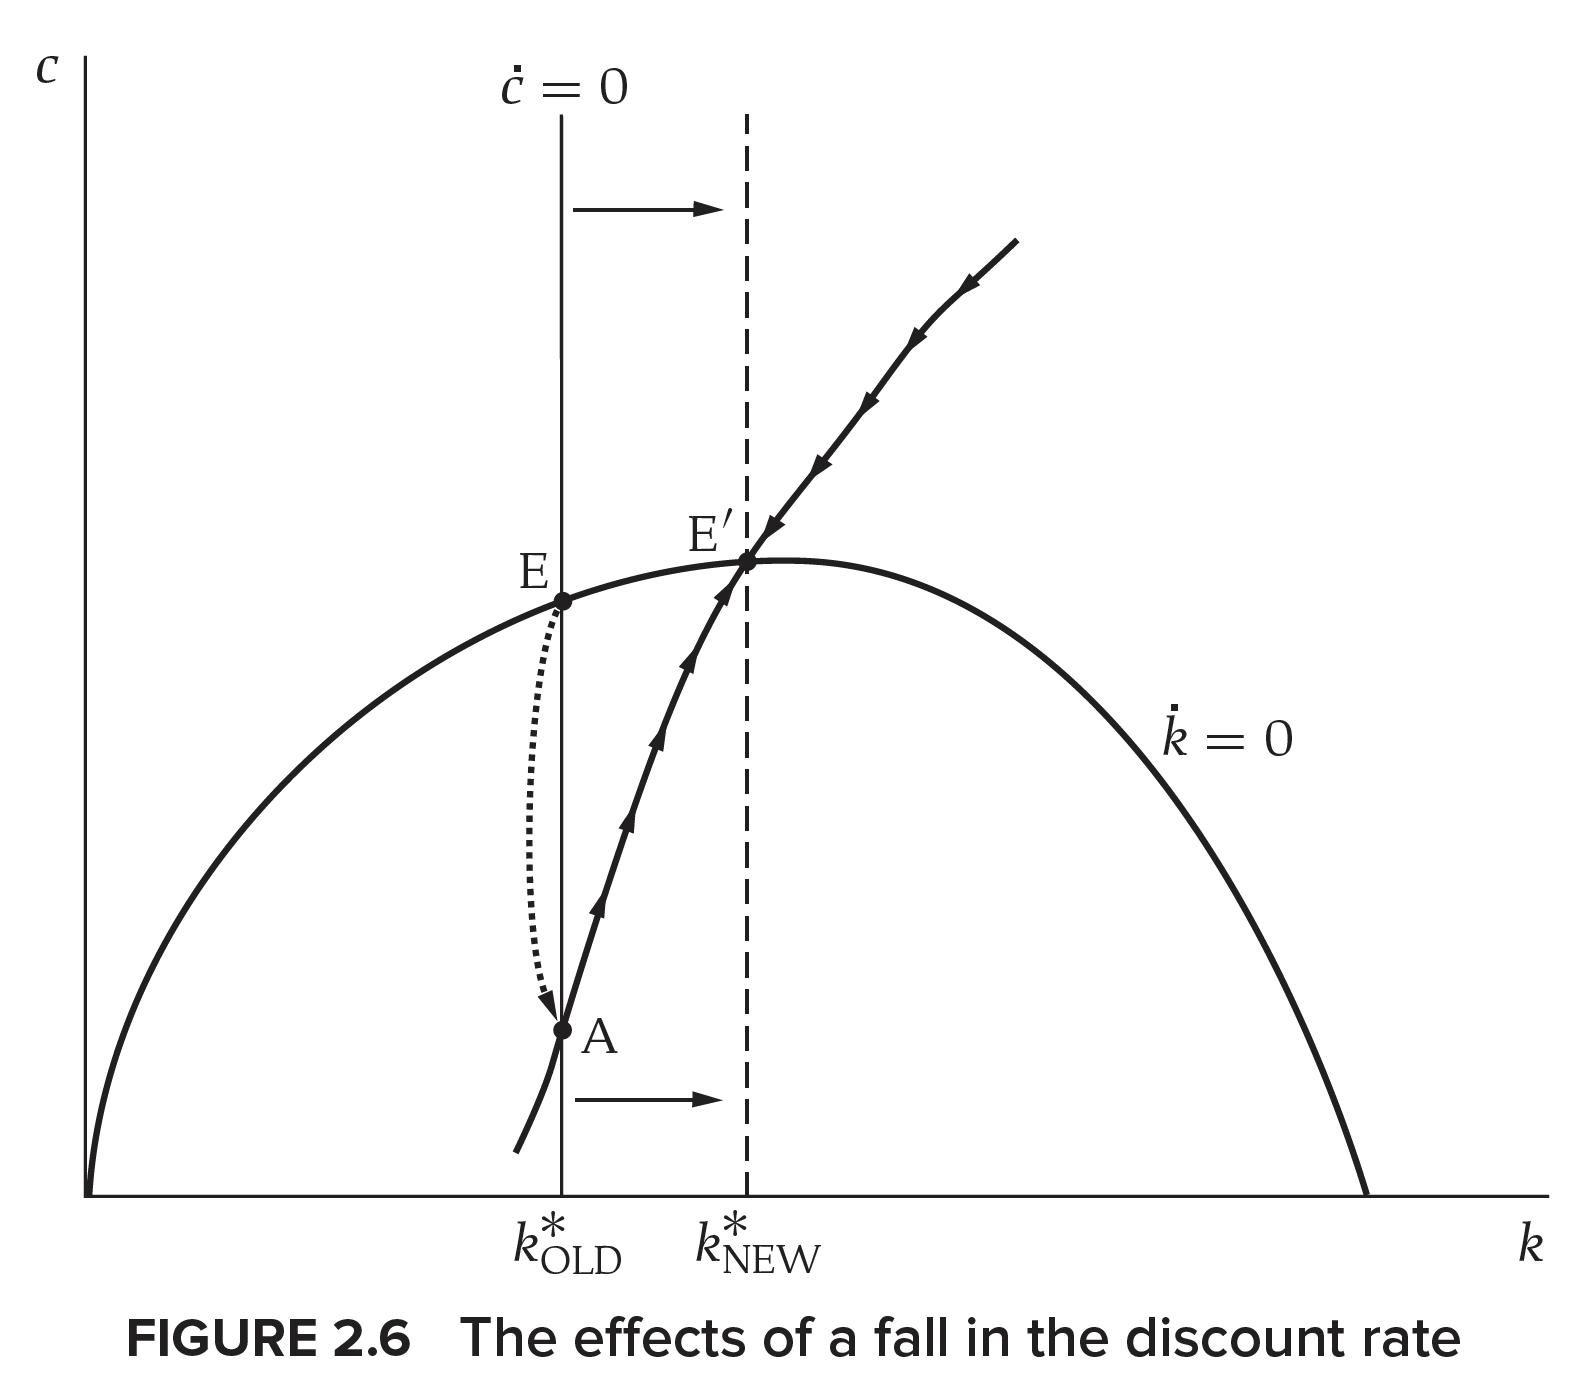
\includegraphics[width=0.6\linewidth]{figures/7_1}
			\end{figure*}
			
			\begin{remark}[Result]
				$c$ jump down so that the economy is on the new saddle path (point $A$), and then the economy moves along the new saddle path till $E'$.
				
				
				\hl{The effects of a fall in $\rho$ are similar to the effects of a rise in the saving rate in the Solow model with a capital stock below the golden-rule level}.
			\end{remark}	
		
		\subsection{Experiment: The Effects of Government Purchases}
			\begin{assumption}
				Assume the government buys output at a rate of $G(t)$ per unit of effective labor.\\
				Further, assuming government expenditure has following 3 properties:
				\begin{enumerate}
					\item Government purchases are assumed \hl{not to affect utility from private consumption}. This can occur if
					\begin{enumerate}
						\item the government devotes the expenditure to an activity consumers don't care about, 
						\item or utility equals the sum of utility from private consumption and utility from government provided goods.
					\end{enumerate}
					\item \hl{not to affect future output}, i.e. the government denotes expenditure to public consumption rather than public investment.
					\item We will find government purchases with \hl{lump-sum} taxes and the government runs a \hl{balanced budget}, that's
					\[
						G(t) = T(t),\ \forall t \in [0, \infty)
					\]
					\end{enumerate}
			\end{assumption}
			\paragraph{Impact}No impact on the $\dot{c} = 0$ curve since the household problem still gives us $\frac{\dot{c}}{c} = \frac{f'(k)-\rho-\theta g}{\theta}$. \\
			However, there is a change in the $\dot{k}=0$ curve, because 
			\begin{equation}
				\dot{k}(t) = y(t) - c(t) - (n+g)k(t) - G(t)
			\end{equation}
			To see there is not effect on $\dot{c}=0$ curve, we need to look at the household's problem. \\
			Let's assume that the Household does not care about $G(t)$. So
			\[
				U = B\int_{t=0}^\infty e^{-\beta t} \frac{c^{1-\theta}}{1-\theta}\ dt
			\]
			And the change comes in the \emph{budget constraint}. Here when we found government expenditure period by period with lump-sum taxes, the government sets tax equal expenses. (Government runs a balanced budget every period.)
			\[
				T(t)A(t)L(t) = G(t)A(t)L(t)
			\]
			The Household's budget constraint then becomes 
			\begin{gather}
				\int_{t=0}^\infty e^{-R(t)} c(t)\frac{A(t)L(t)}{H}\ dt + \int_{t=0}^\infty e^{-R(t)} T(t) \frac{A(t)L(t)}{H}\ dt \leq \frac{K(0)}{H} + \int_{t=0}^\infty e^{-R(t)} w(t) \frac{A(t)L(t)}{H}\ dt
			\end{gather}
			Effectively two means that in terms of the per unit of effective labor variable we got 
			\begin{gather}
				\int_{t=0}^\infty e^{-R(t)} c(t) e^{(n+g)t}\ dt + \int_{t=0}^\infty e^{-R(t)} T(t) e^{(n+g)t}\ dt \leq k(0) + \int_{t=0}^\infty e^{-R(t)} w(t) e^{(n+g)t} \ dt
			\end{gather}
			Given $G(t) = T(t),\ \forall t$, equivalently
			\begin{gather}
				\int_{t=0}^\infty e^{-R(t)} c(t) e^{(n+g)t}\ dt + \int_{t=0}^\infty e^{-R(t)} G(t) e^{(n+g)t}\ dt \leq k(0) + \int_{t=0}^\infty e^{-R(t)} w(t) e^{(n+g)t} \ dt
			\end{gather}
			This means the household's problem can be written as 
			\begin{gather}
				\max_{\{c(t)\}} B\int_{t=0}^\infty e^{-\beta t} \frac{c^{1-\theta}}{1-\theta}\ dt \\
				s.t. \int_{t=0}^\infty e^{-R(t)} c(t) e^{(n+g)t}\ dt + \int_{t=0}^\infty e^{-R(t)} G(t) e^{(n+g)t}\ dt \leq k(0) + \int_{t=0}^\infty e^{-R(t)} w(t) e^{(n+g)t} \ dt
			\end{gather}
			And the Lagrangian becomes
			\begin{gather}
				\mc{L} = B \int_{t=0}^\infty e^{-\beta t} \frac{c^{1-\theta}}{1-\theta}\ dt \\
				+ \lambda \Big[ k(0) + \int_{t=0}^\infty e^{-R(t)} w(t) e^{(n+g)t} \ dt - \int_{t=0}^\infty e^{-R(t)} c(t) e^{(n+g)t}\ dt + \int_{t=0}^\infty e^{-R(t)} G(t) e^{(n+g)t}\ dt\Big]
			\end{gather}
			By solving for the first order condition w.r.t. $c(t)$ we have 
			\[
				\pd{\mc{L}}{c(t)} = B e^{\beta t} c^{-\theta} - \lambda e^{-R(t)} e^{(n+g)t} = 0
			\]
			Since the changing in $G$ does not impact the firms problem we still have $r(t) = f'(k(t))$.
			So at equilibrium we still have 
			\[
				\frac{\dot{c}(t)}{c(t)} = \frac{f'(k(t)) - \rho - \theta g}{\theta}
			\]
			
			\subsubsection{Permanent Change in Government Purchases}
			\paragraph{}Consider a shock that \emph{permanently} increases $G(t)$ from $G_L$ to $G_H$.
			
			\paragraph{Effect} $\frac{\dot{c}}{c}$ locus is not affected, but $\dot{k}=0$ locus shifts down by $\Delta G$. And \hl{$c^*$ falls by $\Delta G$ but $k^*$ does not change}.
			\begin{figure*}[h]
				\centering
				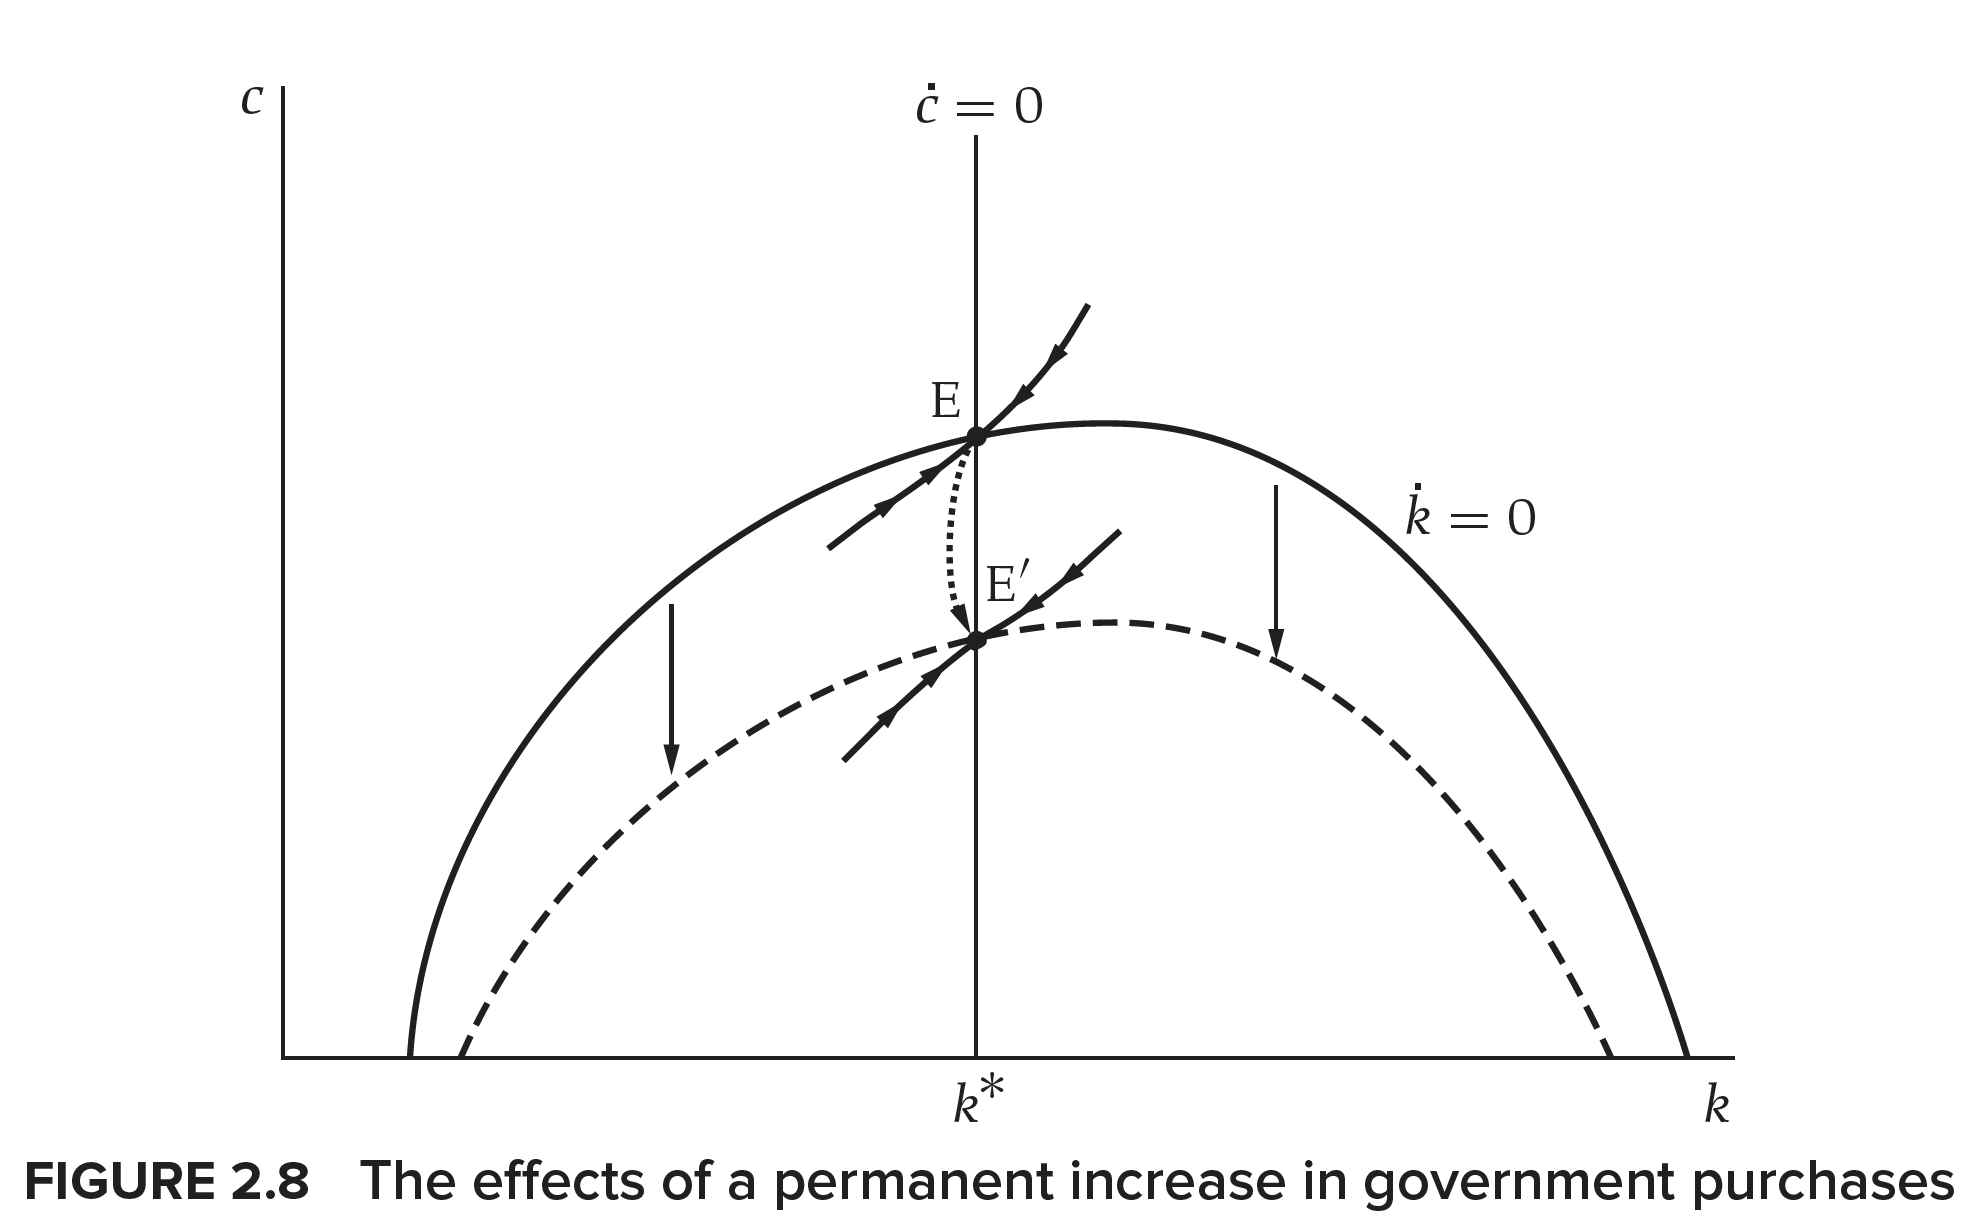
\includegraphics[width=0.8\linewidth]{figures/7_2}
			\end{figure*}
			Optimally, at the time of the shock, the economy jumps from point $E$ (before) to point $E_1$. We move \ul{immediately} from one steady state to the other. (Since no smoothing could be done here) \\
			Since there's no change in $k^*$, there's no change in the rate of return on capital ($f'(k)$) and interest rate.
		
			\subsubsection{Temporary Change in Government Purchases}
			\paragraph{} Assume there's a temporal increase in $G$ and the terminal date is known with certainty. In this case, \hl{$c$ does not fall by the full amount of increase in $G$}. Cause if it did, consumption would jump discontinuously at the time that government purchases return to the original level. \hl{$c$ must jump to the value such that the dynamics implied by $\dot{k}(t) = y(t) - c(t) - (n+g)k(t) - G_H$ bring the economy to the old saddle path at the time that $G$ returns to its initial level}. And $r$ rises gradually during the period that government spending is high and then gradually returns to its initial level.
				\begin{figure*}[h]
					\centering
					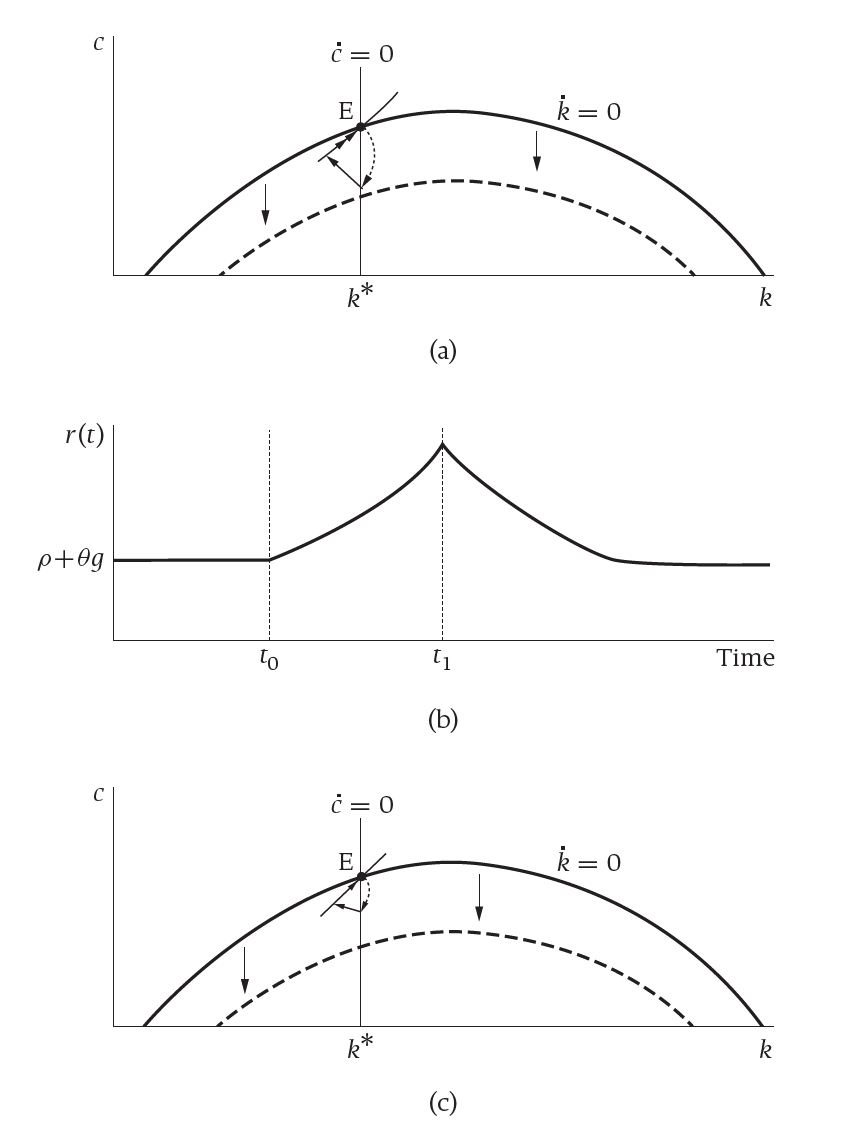
\includegraphics[width=0.7\linewidth]{figures/8_1}
					\caption{The effects of a temporary increase in government purchases}
				\end{figure*}
		\subsection{Extension: Change in Capital Depreciation}
			\par With capital depreciation, Euler equation of consumption and state equation of capital would become
			\begin{gather}
				\frac{\dot{c}}{c} = \frac{f'(k)-\delta-\rho-\theta g}{\theta} \\
				\dot{k} = f(k) - (n+g+\delta)k - c - G
			\end{gather}
			Consider a fall in $\delta$, $k^*$, $k^{GR}$ and $c^*$ all increase with certainty. Immediately after shock, $c$ jumps discourteously onto the new saddle path towards the new steady state. \hl{Note that we have to consider 3 cases when both loci changes, the corresponding $c$ of $k_0$ on new saddle path is above $c_0$, just at $c_0$ or below $c_0$. The immediate behaviour of $c$ differs in those cases.}
			\begin{remark}
				$k$ can only change gradually, and the direction of the immediate discontinuous jump of $c$ depends on the new saddle path.
			\end{remark}
			\begin{remark}
				Change in $g$ and non-parallel change in $f$ would deal similar effect on the phase diagram.
			\end{remark}
			
	\newpage
	\section{Lecture 8 Nov. 1 2018}
		\subsection{Government Spending: without bonds}
			\begin{notation}
				Let $G(t)$ and $T(t)$ denote the government expenditure and taxation (in form of lump-sum tax) per \hl{effective unit of labor} at time period $t$.
			\end{notation}
			
			\begin{assumption}
				Government satisfies its budget constraint in every period,
				\begin{equation}
					G(t) A(t) L(t) = T(t) A(t) L(t)\quad \forall t \in [0, \infty)
				\end{equation}
			\end{assumption}
			
			\paragraph{Household budget} constraint (normalized by $\frac{A(0)L(0)}{H}$) can be expressed as
			\begin{gather}
				k(0) + \int_{t=0}^\infty {e^{-R(t)} e^{(n+g)t} [w(t) - c(t) - T(t)]}\ dt \geq 0 \\
				\iff k(0) + \int_{t=0}^\infty {e^{-R(t)} e^{(n+g)t} [w(t) - c(t) - \textcolor{red}{G(t)}]}\ dt \geq 0
			\end{gather}
			
			\paragraph{State equation} 
			\begin{equation}
				\dot{k}(t) = f(k(t)) - c(t) - G(t) - (n+g)k(t)
			\end{equation}
		
		\subsection{Government Spending: with bonds (voluntary taxation)}
			\paragraph{Household Budget Constraint}
				\begin{equation}
					k(0) + b(0) + \int_{t=0}^\infty {e^{-R(t)} e^{(n+g)t} [w(t) - c(t) - T(t)]}\ dt \geq 0
				\end{equation}
				where government bonds $b(0)$ is considered as a part of \emph{initial asset} of households.
			\paragraph{Government Budget Constraint}
				\begin{gather}
					-b(0) A(0) L(0) + \int_{t=0}^\infty e^{-R(t)} A(t)L(t) [T(t) - G(t)]\ dt \geq 0 \\
					\implies -b(0) + \int_{t=0}^{\infty} e^{-R(t)} e^{(n+g)t} [T(t) - G(t)]\ dt \geq 0 \\
					\tx{With }b(s)e^{(n+g)s} := b(0)e^{R(s)} - \int_{t=0}^{\infty} e^{-R(t)+R(s)} e^{(n+g)t} [T(t) - G(t)]\ dt\\
					\iff \lim_{s\to \infty} b(s) e^{(n+g)s} e^{-R(s)} \textcolor{red}{\leq} 0
				\end{gather}
				Above constraint can be rewritten as \textbf{flow constraint}
				\begin{gather}
					\dot{B}(t) = r(t)B(t) + G(t)A(t)L(t) -T(t)A(t)L(t) \\
					\iff \dot{b}(t) = r(t)b(t) + G(t) - T(t) - (n+g)b(t)
				\end{gather}
			\begin{proposition}
				The effects of government spending on household optimization are the same with and without bonds.
			\end{proposition}
				\begin{proof}
					Adding household budget (5) and government budget (7)
				\begin{gather}
					k(0) + \int_{t=0}^\infty {e^{-R(t)} e^{(n+g)t} [w(t) - c(t) - G(t)]}\ dt \geq 0
				\end{gather}
				Note that (10) is identical to the household budget constraint (3) in last section and taxation and bonds are assumed not affecting household's utility. Therefore household's optimization problem is unchanged under two taxation schemes.
				\end{proof}
				
			\begin{assumption}[Perfect Financial Institute]
				Government and household are facing the same interest rate $r(t)$.
			\end{assumption}
				
			\begin{proposition}[Ricardian Equivalence]
				\emph{Path of taxation} does not affect household behaviour, only \emph{path of government expenditure} does.
			\end{proposition}
			
		\subsection{Problems of Ricardian Equivalence}
			\subsubsection{Turn Over of Population}
				\begin{itemize}
					\item Old people die before high taxes.
					\item Remedies: \textbf{Intergenerational Altruism} generations behave as if they are one infinitely living individual.
				\end{itemize}
				
			\subsubsection{Liquidity Constraint}
				\begin{itemize}
					\item People cannot borrow earlier. (Imperfect financial market)
					\item Response: Government can save for individuals.
				\end{itemize}
			
			\subsubsection{No Lump-sum Tax in Real World}
				\par One critical assumption for Ricardian Equivalence to hold is the tax is flat. But in real world, taxation (e.g. consumption tax) can introduce significant distortion to household budget constraint and thus household behaviour.
				
			\subsubsection{Rule of Thumb: Imperfect Foreseeing}
				\par People cannot foresee future events perfectly, instead, they follow rule of thumb (e.g. same 20\% of income). Therefore they do not always act optimally.
				
	\section{Lecture 9 Nov. 22 2018}
		\subsection*{Business Cycles}
			\par \textbf{Potential causes of business cycles}
			\begin{itemize}
				\item Technology shocks.
				\item \st{Monetary policy shocks. (e.g. Fed unexpected changed something)}
				\item Government shocks.
			\end{itemize}
		\subsection{Business Cycle Facts}
			\begin{enumerate}
				\item Fluctuations do not exhibit any simple regular or cyclical pattern.
				\item Fluctuations are distributed every \ul{unevenly} over \ul{components of output}. \footnote{i.e. consumption, investment, government expenditure and exports.} \begin{itemize}
						\item \emph{\ul{Investment} (primarily inventories) fluctuates more than consumption}.	
 						\end{itemize}
				\item There are no large asymmetries between rises and falls in output (i.e. \emph{output growth is distributed roughly symmetrically around its mean}). But there are asymmetries in terms of timing.
				\item In a recession,
					\begin{enumerate}
						\item real GPD
						\item employment
						\item weekly hours in manufacturing
						\item interest rates and inflation		
					\end{enumerate} \emph{typically} fall.
				\item Decline in employment and hours are generally smaller than the fall in output.
					\begin{itemize}
						\item \textbf{Okun's Law}: a short fall in GPD of 2 percentage relative to normal growth produces a 1 percentage rise in unemployment.
					\end{itemize}
				\item Productivity (\textcolor{red}{$:=\frac{output}{worker\ hours}$}) declines in a recession.
			\end{enumerate}
			
			\begin{definition}
				A \textbf{Walrasian model} is a \hl{competitive} model (i) without externalities, (ii)asymmetric information, (iii)missing markets (i.e. complete) or other imperfections.
			\end{definition}
		\subsection{Baseline Business Cycle Model}
			\par A discrete time version of the Ramsey-Cass-Koopman model.
			\paragraph{Firms} produce using the production function
			\begin{equation}
				Y_t = K_t^\alpha (A_t L_t)^{1-\alpha},\ \alpha \in (0,1)
			\end{equation}
			where $A_t$ is the knowledge or technology at time $t$, $K_t$ is the amount of capital rented at time $t$, $L_t$ is the amount of labor hired at time $t$.
			\begin{remark}
				Note that in RBC model, people supply a friction of their time endowment, $\ell$, to the labor market, so 
				\[
					L_t \leq N_t
				\]
			\end{remark}
			
			\paragraph{Output} is divided between consumption and investment and government expenditure.
			\begin{gather}
				Y_t = C_t + I_t + G_t \\
				I_t = K_{t+1} - (1-\delta)K_t
			\end{gather}
			
			\paragraph{Government Purchases} are financed by \ul{lump sum taxes} here.
			\begin{remark}
				Ricardian Equivalence suggests even government finances its expenditure with bonds, the main implication of this model will not change.
			\end{remark}
			
			\paragraph{Ricardian Equivalence} Since households are infinitely lived and there are no capital market imperfection, Ricardian Equivalence holds in the baseline model.
			
			\subsubsection{Firm's Problem}
				\par Firms maximize the \ul{net profits}.
				\begin{gather}
					\max_{K_t, L_t} Y_t - \delta K_t - w_t L_t - r_t K_t
				\end{gather}
				where $Y_t - \delta K_t$ is the \textbf{net production function}. Substitute in equation (1),
				\begin{gather}
					\max_{K_t, L_t} K_t^\alpha (A_t L_t)^{1-\alpha} - \delta K_t - w_t L_t - r_t K_t
				\end{gather}
				First order conditions are given as
				\begin{gather}
					K_t:\quad \alpha K_t^{\alpha - 1} (A_t L_t)^{1-\alpha} - \delta - r_t = 0 \\
					L_t:\quad (1-\alpha) K_t^\alpha A_t ^{1-\alpha} L_t^{-\alpha} - w_t = 0
				\end{gather}
				\begin{remark}
					Equivalently, FOC can be expressed with the intensive-form production function,
					\begin{gather}
						r_t = f'(k_t) - \delta\\
						w_t = A_t [f(k_t) - k_t f'(k_t)]
					\end{gather}
				\end{remark}
			\subsubsection{Households}
				\par Households are \ul{infinitely lived} and there are $H$ households in the economy, $H$ is large.
				\paragraph{Population} grows exogenous at rate $n$,
					\begin{equation}
						\ln N_t = \overline{N} + nt,\quad n < \rho
					\end{equation}
				The representative household maximizes the \hl{expected} value of
				\begin{equation}
					\expat{0}{\sum_{t=0}^\infty e^{-\rho t} u(c_t, 1- \ell_t) \frac{N_t}{H}}
				\end{equation}
				where $c_t$ is the consumption \emph{per member} of the household and $1-\ell_t$ is the \emph{fraction} of time that the household devotes to leisure.
				\begin{remark}
					Another way of interpreting $1-\ell_t$ is that the actual amount of the \emph{time endowment} is normalized to 1.
				\end{remark}
				\par $u(\cdot)$ is the \emph{instantaneous utility function} of a member.
				\par Since all households are the same, the total amount of consumption and labor supplied at equilibrium is
				\begin{gather}
					C_t = c_t N_t \\
					L_t = \ell_t N_t
				\end{gather}
				And 
				\begin{equation}
					\expat{t}{\sum_{t=0}^\infty e^{-\rho t} u(c_t, 1- \ell_t) \frac{N_t}{H}}
				\end{equation}
				is the expectation of lifetime utility at date $t$.
				\par Assume each household has $\frac{K_0}{H}$ unit of wealth at the beginning date. \\
				Also assuming the instantaneous utility function is log-separable
				\begin{equation}
					u(c_t, 1-\ell_t) = \ln c_t + b \ln(1-\ell_t),\ b > 0
				\end{equation}
			\subsubsection{Technology Shocks}
				\par Assuming
				\begin{equation}
					\ln A_t = \overline{A} + gt + \tilde{A}_t
				\end{equation}
				where $\tilde{A}_t$ is a \emph{first order auto-regressive process}
				\begin{equation}
					\tilde{A}_t = \rho_A \tilde{A}_{t-1} + \epsilon_{A, t}\quad \rho_A \in (-1, 1)
				\end{equation}
				where $\epsilon_{A,t}$ follows a \emph{white-noise} disturbance.
			
			\begin{definition}
				A \textbf{white-noise disturbance} are a series of mean zero shocks that are uncorrelated with one another.
			\end{definition}
			
			\begin{remark}
				$\rho_A$ measures the \emph{persistence} at a shock since $\tilde{A}_t$ is a fraction at last period's value plus the shock.
			\end{remark}
			\begin{assumption}
				We assume $\rho_A > 0$ since we are assuming no oscillation.
			\end{assumption}
			
		\subsubsection{Government Shock}
			\par To caputre trend growth in government expenditures, we assume in absence of shocks
			\begin{equation}
				\ln G_t = \overline{G} + (g+n)t
			\end{equation}
			where $g$ is the rate of technical progress and $n$ is the rate of population growth.
			
			\begin{remark}
				Note that on the balanced growth path, $Y_t$ grows at a constant rate of $n+g$. The growth rate $n+g$ of $G$ guarantees the fraction of $G_t$ relative to $Y_t$ is not vanishing or exploding as $t \to \infty$.
			\end{remark}
			With shocks we have
			\begin{equation}
				\ln G_t = \overline{G} + (g+n)t + \tilde{G}_t
			\end{equation}
			where $\tilde{G}_t$ is a first order auto-regressive process
			\begin{equation}
				\tilde{G}_t = \rho_G \tilde{G}_{t-1} + \epsilon_{G,t}\quad \rho_G \in (-1,1)
			\end{equation}
			where $\epsilon_{G,t}$ are white-noise disturbance.
			
			\subsection{Case 1}
				\paragraph{Assumptions} Households live one period, there is no uncertainty no initial wealth and one person per household and no growth.
				\paragraph{Budget} $c \leq w \ell$
				\paragraph{Household's Problem}
				\begin{gather}
					\max_{c, \ell} \ln c + b \ln (1-\ell) \\
					s.t.\ c \leq w\ell
				\end{gather}
				\paragraph{Solving the model} Setup the Lagrangian,
				\begin{equation}
					\mc{L}(\cdot) = \ln c + b \ln (1-\ell) + \lambda (w \ell - c)
				\end{equation}
				First order conditions
				\begin{gather}
					\begin{cases}
						\pd{\mc{L}}{c} = \frac{1}{c} - \lambda = 0 \\
						\pd{\mc{L}}{\ell} = \frac{-b}{1-\ell} + w \lambda = 0 \\
						\pd{\mc{L}}{\lambda} = w\ell - c = 0
					\end{cases} \\
					\implies \frac{1}{c} w = \frac{b}{1-\ell} \\
					\implies \ell = \frac{1}{1+b} < 1
				\end{gather}
			
			\subsection{Case 2}
				\paragraph{Assumptions:}
					\begin{enumerate}
						\item Household lives for 2 periods
						\item No growth
						\item No uncertainty
						\item No initial wealth
						\item One person per family/household
					\end{enumerate}
				\paragraph{Budget Constraint}
					\begin{equation}
						c_0 + \frac{c_1}{1+r} \leq w_0 \ell_0 + \frac{w_1 \ell_1}{1+r}
					\end{equation}
				
				\paragraph{Household's Problem}
					\begin{gather}
						\max_{\{c_0, c_1, \ell_0, \ell_1\}} \ln c_0 + b \ln (1-\ell_0) + e^{-\rho} (\ln c_1 + b \ln (1-\ell_1))\\
						s.t.\ c_0 + \frac{c_1}{1+r} \leq w_0 \ell_0 + \frac{w_1 \ell_1}{1+r}
					\end{gather}
				
				\paragraph{Solving the model} Setup the Lagrangian
					\begin{equation}
						\mc{L}(\cdot) = \ln c_0 + b \ln (1-\ell_0) + e^{-\rho} (\ln c_1 + b \ln (1-\ell_1)) + \lambda \Big(w_0 \ell_0 + \frac{w_1 \ell_1}{1+r} - c_0 - \frac{c_1}{1+r} \Big)
					\end{equation}
					First order conditions
					\begin{gather}
							\pd{\mc{L}}{c_0} = \frac{1}{c_0} - \lambda = 0 \\
							\pd{\mc{L}}{c_1} = e^{-\rho} \frac{1}{c_1} - \lambda (\frac{1}{1+r}) = 0 \\
							\pd{\mc{L}}{\ell_0} = \frac{-b_0}{1-\ell_0} + w_0 \lambda = 0 \\
							\pd{\mc{L}}{\ell_1} = e^{-\rho}(\frac{-b_0}{1-\ell_1}) + \frac{w_1}{1+r}\lambda = 0 \\
							\pd{\mc{L}}{\lambda} = c_0 + \frac{c_1}{1+r} - w_0 \ell_0 - \frac{w_1 \ell_1}{1+r} = 0
					\end{gather}
					\paragraph{Intra-temporal Trade-offs}
						Therefore, (22) and (24) imply
						\begin{equation}
							\frac{w_0}{c_0} = \frac{b}{1-\ell_0}
						\end{equation}
						and (23) and (25) implies
						\begin{equation}
							\frac{w_1}{c_1} = \frac{b}{1-\ell_1}
						\end{equation}
					\paragraph{Inter-temporal Trade-offs}
						(22) and (23) imply
						\begin{equation}
							\frac{1}{c_0} = e^{-\rho}(1+r)\frac{1}{c_1}
						\end{equation}
						Note that the two sides of equation (29) are the discounted marginal utilities.
						(24) and (25) together imply
						\begin{equation}
							\frac{1-\ell_0}{1-\ell_1} = \frac{w_1}{w_0}\frac{1}{e^{-\rho}(1+r)}
						\end{equation}
					\paragraph{Observation 1} If $w_0$ rises relative to $w_1$, then $\frac{w_1}{w_0}$ falls. Keeping everything else equal, $\frac{1-\ell_0}{1-\ell_1}$ falls.
					\paragraph{Observation 2} If $\rho$ increases, then $\frac{1}{e^{\rho}(1+r)}$ increases. Then $\frac{1-\ell_0}{1-\ell_1}$ increases.
					\paragraph{Observation 3} If $r$ increases, then $\frac{1-\ell_0}{1-\ell_1}$ falls.
					\paragraph{Observation 4} The \textbf{inter-temporal  elasticity of substitution} between leisure in the two periods equals one.
					\begin{proof}
						\begin{gather}
							\pd{1-\ell_0}{1-\ell_1} \cdot \frac{1-\ell_1}{1-\ell_0} \\
							= \frac{w_1}{w_0} \frac{1}{e^{-\rho}(1-r)} \frac{1-\ell_1}{1-\ell_0} \\
							= \frac{1-\ell_0}{1-\ell_0} = 1
						\end{gather}
					\end{proof}
	\section{Lecture 10 Nov. 29 2018}
		\subsection{Case 3}
			\begin{assumption} \quad
				\begin{enumerate}
					\item No uncertainty 
					\item One member per household
					\item No depreciation ($\delta = 0$)
					\item No growth
					\item Infinite time horizon
					\item Only one single household in the economy $H=1$
				\end{enumerate}
			\end{assumption}
			
			\subsubsection{Setup the Model}
			\paragraph{Objective Function}
				\begin{equation}
					\sum_{t=0}^\infty e^{-\rho t} [\ln(c_t) + b\ln(1-\ell_t)]
				\end{equation}
			
			\paragraph{Controls} Individual households choose 
				\begin{itemize}
					\item \ul{Consumption} $c_t$
					\item \ul{Leisure} $\ell_t$
					\item and \ul{Saving} $K_{t+1}$
				\end{itemize}
			\paragraph{Budget Constraint} At each time period $t$,
			\begin{equation}
				K_{t+1} - K_t + c_t + G_t \leq r_t K_t + w_t \ell_t
			\end{equation}
			where $I_{t} = K_{t+1} - K_t$ since there's on depreciation.
			
			\subsubsection{Solving the Model}
			\paragraph{Lagrangian}
			\begin{gather}
				\mc{L} = \sum_{t=0}^\infty \Big\{e^{-\rho t} [\ln(c_t) + b\ln(1-\ell_t)]
				+ \lambda_t [r_t K_t + w_t \ell_t - K_{t+1} + K_t - c_t - G_t] \Big\}
			\end{gather}
			\paragraph{First Order Conditions}\hl{have to be satisfied at every time period $t \in \R_{\geq 0}$}
			\begin{gather}
				\pd{\mc{L}}{c_t} = e^{-\rho t}\frac{1}{c_t} - \lambda_t = 0,\quad \forall t \in \R_+ \\
				\pd{\mc{L}}{\ell_t} = e^{-\rho t} \frac{-b}{1-\ell_t} + \lambda_t w_t = 0,\quad \forall t \in \R_+ \\
				\pd{\mc{L}}{K_{t+1}} = -\lambda_t + (1+r_{t+1})\lambda_{t+1} = 0,\quad \forall t \in \R_+ \\
				\pd{\mc{L}}{\lambda_t} = r_t K_t + w_t \ell_t - K_{t+1} + K_t - c_t - G_t = 0,\quad \forall t \in \R_+
			\end{gather}
			\begin{remark}
				Equation (4) implies $\lambda_t > 0,\quad \forall t \in \R_+$, so KTT complementary slackness condition suggests budget constraint are hold as equalities at each time $t$.
			\end{remark}
			
			\subsubsection{Analysis}
			
			\paragraph{Inter-Temporal Consumption}
				\begin{gather}
					\begin{cases}
						\pd{\mc{L}}{c_t} = 0 \iff \lambda_t = e^{-\rho t}\frac{1}{c_t} \\
						\pd{\mc{L}}{c_{t+1}} = 0 \iff \lambda_{t+1} = e^{-\rho (t+1)}\frac{1}{c_{t+1}} \\
						\lambda_t = \lambda_{t+1}(1+r_{t+1})
					\end{cases}\\
					\iff \frac{1}{c_t} = (1+r_{\textcolor{red}{t+1}})e^{-\rho}\frac{1}{c_{t+1}}
				\end{gather}
				
			\paragraph{Intra-Temporal Consumption-Leisure}
				\begin{gather}
					\begin{cases}
						\pd{\mc{L}}{\ell_t} = 0 \iff e^{-\rho t} \frac{b}{1-\ell_t} = \lambda_t w_t \\
						\pd{\mc{L}}{c_t} = 0 \iff \lambda_t = e^{-\rho t}\frac{1}{c_t}
					\end{cases} \\
					\iff e^{-\rho t} \frac{b}{1-\ell_t} = e^{-\rho t}\frac{1}{c_t} w_t \\
					\iff \frac{b}{1-\ell_t} = \frac{1}{c_t} w_t,\quad \forall t \in \R_+
				\end{gather}
				
			\paragraph{Inter-Temporal Leisure}
				\begin{gather}
					\begin{cases}
						\pd{\mc{L}}{\ell_t} = 0 \iff e^{-\rho t} \frac{b}{1-\ell_t} = \lambda_t w_t \\
						\pd{\mc{L}}{\ell_{t+1}} = 0 \iff e^{-\rho (t+1)} \frac{b}{1-\ell_{t+1}} = \lambda_{t+1} w_{t+1} \\
						\pd{\mc{L}}{K_{t+1}} = 0 \iff \lambda_t = (1+r_{t+1})\lambda_{t+1}
					\end{cases}\\
					\implies \frac{b}{1-\ell_t} \frac{1}{w_t} = e^{-\rho} (1+r_{t+1}) \frac{b}{1-\ell_{t+1}}\frac{1}{w_{t+1}} \\
					\iff \frac{1-\ell_{t}}{1-\ell_{t+1}} = \frac{w_{t+1}}{w_{t}} \frac{1}{(1+r_{t+1}) e^{-\rho}}
				\end{gather}
			\begin{remark}
				Above results on optimality conditions (i.e. inter-temporal substitutes and intra-temporal substitutions) are the same as in previous two period case (case 2).
			\end{remark}	
		\subsection{Case 4}
			\begin{assumption}
				Add \textbf{uncertainty} to case 3.
			\end{assumption}
		\subsubsection{Setup the Model}
			\paragraph{Budget Constraint at $t$}
			\begin{equation}
				K_{t+1} - K_t + c_t + G_t \leq w_t \ell_t + r_t K_t
			\end{equation}
			\paragraph{(Optional)} if we relax the assumption $\delta = 0$, the budget constraint becomes
			\begin{equation}
				K_{t+1} - K_t + c_t + G_t \leq w_t \ell_t + r_t K_t
			\end{equation}
		\subsubsection{Solving the Model}
			\paragraph{Lagrangian}
			\begin{equation}
				\mc{L} = \expat{\textcolor{red}{0}}{\sum_{t=0}^\infty e^{-\rho t}[\ln(c_t) + b \ln(1-\ell_t)] + \lambda_t [w_t \ell_t + r_t K_t - c_t - K_{t+1} + K_t - G_t]}
			\end{equation}

			\begin{remark}
				\[
					\expat{t}{\lambda_t} = \lambda_t
				\]
				No uncertainty presents in the \ul{shadow price}, $\lambda_t$, for any given time period $t$. (i.e. we assume individuals know well how they value their extra gain upon relaxing budget constraint a little bit.)
			\end{remark}

			\paragraph{First Order Condition with Expectations}
			For all $t$ and all states of the world,
			\begin{gather}
				\pd{\mc{L}}{c_t} = \expat{\textcolor{red}{t}}{e^{-\rho t}\frac{1}{c_t} - \lambda_t} = 0 \\
				\iff e^{-\rho t} \frac{1}{c_t} = \lambda_t \\
				\pd{\mc{L}}{\ell_t} = \expat{t}{e^{-\rho t} \frac{-b}{1-\ell_t} - \lambda_t w_t} = 0 \\
				\iff e^{-\rho t} \frac{b}{1-\ell_t} = \lambda_t w_t \\
				\pd{\mc{L}}{K_{t+1}} = \expat{t}{-\lambda_t + \lambda_{t+1}(1 + r_{t+1})} = 0 \\
				\iff \lambda_t = \expat{t}{\lambda_{t+1}(1+r_{t+1})} \\
				\pd{\mc{L}}{\lambda_t} = 0 \iff K_{t+1} - K_t + c_t + G_t = w_t \ell_t + r_t K_t
			\end{gather}
		\subsubsection{Analysis}
			\paragraph{Intra-Temporal Consumption-Leisure}
			\begin{equation}
				\frac{b}{1-\ell_t} = w_t\frac{1}{c_t}
			\end{equation}
			
			\paragraph{Inter-Temporal Consumption}
			\begin{gather}
				\frac{1}{c_t} = e^{-\rho} \expat{t}{(1 + r_{t+1})\frac{1}{c_{t+1}}} \\
				\equiv e^{-\rho} \expat{t}{1+r_{t+1}-\delta}\expat{t}{\frac{1}{c_{t+1}}} + e^{-\rho} Cov(1+r_{t+1}-\delta, \frac{1}{c_{t+1}})
			\end{gather}
			
			\paragraph{Inter-Temporal Leisure}
			\begin{gather}
				e^{-\rho t} \frac{b}{(1-\ell_t) w_t} = e^{-\rho (t+1)} \expat{t}{\frac{b}{(1-\ell_{t+1})w_{t+1}} (1 + r_{t+1})} \\
				\implies \frac{1}{1-\ell_t} \frac{1}{w_t} = e^{-\rho} \expat{t}{\frac{1}{1-\ell_{t+1}}\frac{1}{w_{t+1}} (1 + r_{t+1})}
			\end{gather}
		\subsection{Social Planner Problem}
			\par The social planner maximize household utility subject to aggregate resource constraint. \hl{We are going to show the solutions to social planner problem and decentralized household optimization problem collides }
			\begin{assumption}
				For simplicity, $\delta=0$ and there's no growth, population is fixed at $N$. Further assuming the production function is in Cobb-Douglas Form.
			\end{assumption}
		\subsubsection{Setup the Model}
			\paragraph{Optimization}
			\begin{gather}
				\max_{\{c_t, \ell_t, K_{t+1}\}_{t=0}^\infty} \expat{\textcolor{red}{0}}{\sum_{t=0}^\infty e^{-\rho t} [\ln(c_t) + b \ln(1-\ell_t)]\textcolor{red}{N}} \\
				s.t.\ 0 \leq K_t^\alpha (A_t \ell_t N)^{1-\alpha} - Nc_t - K_{t+1} + K_t - G_t
			\end{gather}
		\subsubsection{Solving the Model}
			\paragraph{Lagrangian}
			\begin{equation}
				\mc{L} = \expat{\textcolor{red}{0}}{\sum_{t=0}^\infty e^{-\rho t} [\ln(c_t) + b \ln(1-\ell_t)]\textcolor{red}{N}} + \lambda_t \Big (K_t^\alpha (A_t \ell_t N)^{1-\alpha} - Nc_t - K_{t+1} + K_t - G_t \Big )
			\end{equation}
			
			\paragraph{First Order Necessary Conditions}\hl{for all $t$ and all sates of the world}.
			\begin{gather}
				\pd{\mc{L}}{c_t} = \expat{t}{e^{-\rho t} \frac{1}{c_t}N - \lambda_t N} = 0 \\
				\implies e^{-\rho t} \frac{1}{c_t} = \lambda_t
			\end{gather}
			\begin{gather}
				\pd{\mc{L}}{\ell_t} = \expat{t}{e^{-\rho t} (\frac{-b}{1-\ell_t})N + \lambda_t \Big( (1-\alpha)K_t^\alpha (A_t N)^{1-\alpha} \ell_t ^ {-\alpha}\Big)} = 0 \\
				\implies e^{-\rho t} \frac{b}{1-\ell_t} = \lambda_t \frac{Y_t}{\ell_t N} (1-\alpha)
			\end{gather}
			\begin{gather}
				\pd{\mc{L}}{K_{t+1}} = \expat{t}{-\lambda_t + \lambda_{t+1}\{\alpha K_{t+1}^{\alpha-1}(A_{t+1} \ell_{t+1} N)^{1-\alpha} \textcolor{red}{+ 1}\}} \\
				\implies \lambda_t = \expat{t}{\lambda_{t+1} (\alpha \frac{Y_{t+1}}{K_{t+1}} + 1)}
			\end{gather}
			where $\alpha \frac{Y_{t+1}}{K_{t+1}} + 1$ is the aggregate net return (no depreciation) to capital. ($\alpha$ equals the share of income goes to capital in equilibrium.) \\
			\begin{gather}
				e^{-\rho t} \frac{1}{c_t} = \expat{t}{e^{-\rho(t+1)} \frac{1}{c_{t+1}} (\alpha \frac{Y_{t+1}}{K_{t+1}} + 1)} \\
				\implies \frac{1}{c_t} = e^{-\rho}\expat{t}{\frac{1}{c_{t+1}} (\alpha \frac{Y_{t+1}}{K_{t+1}} + 1)}
			\end{gather}
		\subsubsection{Analysis}
			\begin{remark}
				Perfectly competitive decentralize economy implies no profit and
				\[
					Y_t = r_t K_t + w_t \ell_t N,\quad \forall t \in \R_+
				\]
			\end{remark}
			Also,
			\begin{gather}
				\pd{\mc{L}}{\lambda_t} = 0 
				\implies Y_t = Nc_t + K_{t+1} - K_t + G_t
			\end{gather}
			
			\par Note from the decentralized economy, $\alpha$ and $1 - \alpha$ represents the share of income (aggregate output) to capital and labor respectively.
			\begin{gather}
				w_t = (1-\alpha)\frac{Y_t}{L_t} = (1-\alpha) \frac{Y_t}{\ell_t N} \\
				r_{t+1} = \alpha \frac{Y_{t+1}}{K_{t+1}}
			\end{gather}
			\par So the equilibrium conditions  in the decentralized economy reduce to the same conditions found in the Social Planner's economy in equilibrium. \\
			And \hl{the first welfare theorem holds}.
			
		\subsection{Solving One Model (Optional)}
		\emph{\textbf{Note}: materials below are not required for ECO325}
		\begin{assumption}
			For simplicity, assume \ul{full depreciation}, i.e. $\delta = 1$.
		\end{assumption}
		\paragraph{Note} only focus on two variables for the solution, label supply per person, $\ell$, and fraction of output saved, $s$. Solve the model by checking the \textbf{log-linear} versions of equilibrium conditions and \hl{replace $c_t = \frac{C_t}{N} = (1-s_t)\frac{Y_t}{N_t}$} whenever it appears.
		\begin{gather}
			\frac{1}{c_t} = e^{-\rho} \expat{t}{(1+r_{t+1})\frac{1}{c_t}} \\
			\implies -\ln(c_t) = - \rho_t + \ln \expat{t}{(1+r_{t+1})\frac{1}{c_{t+1}}} \\
			\implies - \ln((1-s_t)\frac{Y_t}{N_t}) = -\rho + \ln(\expat{t}{\frac{\alpha \frac{Y_{t+1}}{K_{t+1}}}{(1-s_{t+1})\frac{Y_{t+1}}{N_{t+1}}}}) \\
			\iff -\ln(1-s_t) + \ln(N_t) - \ln(Y_t) = -\rho + \ln(\alpha) - \ln(K_{t+1}) + \ln(\expat{t}{\frac{N_t e^n}{1-s_{t+1}}}) \\
			= -\rho + \ln(\alpha) - \ln(s_t Y_t) + n + \ln(N_t) \\
			\iff -\ln(1-s_t) = -\rho + n + \ln(\alpha) - \ln(s_t) - \ln(\expat{t}{\frac{1}{1-s_{t+1}}})
		\end{gather}
		Those two implies $s_t = s^*$, i.e. a constant, in equilibrium. \\
		Also we have 
		\begin{gather}
			\frac{b}{1-\ell_t} = \frac{w_t}{c_t} \\
			\implies \ln(b) - \ln(1-\ell_t) = \ln(w_t) - \ln((1-s^*)\frac{Y_t}{N_t}) \\
			= \ln((1-\alpha) \frac{Y_t}{\ell_t N_t}) - \ln(1-s^*) - \ln(Y_t) + \ln(N_t) \\
			= \ln(1-\alpha) - \ln(\ell_t) - \ln(1-s^*)\\
			\implies \ell^* = \frac{1-\alpha}{(1-s)b + (1-\alpha)} < 1
		\end{gather}
		and $\ell_t$ is constant at $\ell^*$ in equilibrium.
		\paragraph{Equilibrium} as we found the equilibrium where $s_t = s^*$ and $\ell_t = \ell^*$ given $A_0, N_0$ and the growth rate. At any $t \in \R_+$,
		\begin{gather}
			\ell_t = \ell^* \\
			L_t = \ell^* N_t \\
			Y_t = K_t^\alpha (L_t A_t) ^{1-\alpha} \\
			K_{t+1} = s^* Y_t \\
			C_t = (1-s^*)Y_t \\
			w_t = (1-\alpha) \frac{Y_t}{L_t} \\
			r_t = \alpha \frac{Y_t}{K_t} - 1.
		\end{gather}
		
		\paragraph{Impulse Response Function} Note that
		\begin{gather}
			\ln(Y_t) = (1 - \alpha) \ln(A_t) + \alpha \ln (K_t) + (1-\alpha) \ln (L_t) \\
			= (1 - \alpha) (\overline{A} + gt + \tilde{A}_t) + \alpha \ln(s Y_{t-1}) + (1-\alpha) \ln(\ell N_t) \\
			= (1 - \alpha) (\overline{A} + gt + \tilde{A}_t) + \alpha \ln (s^*) + \alpha \ln(Y_t) + (1-\alpha) \ln (\ell) + (nt + \overline{N})(1-\alpha) \\
			\implies \ln(\tilde{Y}_t) = (1-\alpha) (\overline{A} + gt) + \alpha \ln(s^*) + \alpha \ln(\tilde{Y}_{t-1}) + (1-\alpha) \ln(\ell) + (nt + \overline{N})(1-\alpha) \\
			\implies \ln(\hat{y}_t) = \ln(Y_t) - \ln(\tilde{Y}_t) \\
			= (1-\alpha)\tilde{A}_t + \alpha \hat{Y}_{t-1} \\
			\implies \frac{\hat{Y}_t - \alpha \hat{Y}_{t-1}}{1-\alpha} = \rho_A (\frac{\hat{Y}_{t-1} - \hat{Y}_{t-2}}{1-\alpha}) + \epsilon_{A, t} \\
			\implies \hat{Y}_{t} = (\rho_A + \alpha) \hat{Y}_{t-1} - \rho_A \alpha \hat{Y}_{t-2} + (1 - \alpha)\epsilon_{A, t}
		\end{gather}
	
	\section{Some Extensions to the Baseline RBC Model}
	\paragraph{} Please note that contents in this section is not covered in lecture.
		\subsection{A More General Case (Optional)}
			\begin{assumption}
				In this general case, all restrictions in previous cases are relaxed.
			\end{assumption}
			
			\begin{notation} Notations used in this section should be consistent with Romer's textbook.
				\textbf{Exogenous Parameters}
					\begin{enumerate}
						\item $\delta :=$ Depreciation rate of capital.
						\item $g :=$ Growth rate of technology.
						\item $n :=$ Growth rate of population.
						\item $\mc{U} :=$ Lifetime utility functional of household.
						\item $\rho :=$ Discount rate of utility.
						\item $\rho_A :=$ AR(1) parameter of technology shocks.
						\item $\rho_G :=$ AR(1) parameter of government shocks.
					\end{enumerate}
				\textbf{Initial Parameters}
					\begin{enumerate}
						\item $A_0 :=$ Initial technology.
						\item $G_0 :=$ Initial capital stock.
						\item $K_0 :=$ Initial aggregate capital in the economy.
						\item $N_0 :=$ Initial population.
					\end{enumerate}
				\textbf{Endogenous Variables}
					\begin{enumerate}
						\item $A_t := $ Technology at time $t$.
						\item $c_t :=$ Consumption per person at time $t$.
						\item $C_t \equiv c_t N_t :=$ Aggregate consumption at time $t$.
						\item $G_t :=$ Aggregate (net) government expenses at time $t$.
						\item $H :=$ A constant representing number of households in the economy.
						\item $K_t :=$ Total amount of capital stock at time $t$.
						\item $L_t \equiv \ell_t N_t :=$ Total labor supply at time $t$.
						\item $\ell_t :=$ Friction of time devoted to labor supply at time $t$.
						\item $N_t :=$ Total population at time $t$.
						\item $r_t :=$ interest rate at time $t$.
						\item $s_t :=$ Saving rate at time $t$.
						\item $Y_t :=$ Aggregate output at time $t$.
					\end{enumerate}
			\end{notation}
		
			
			\setcounter{equation}{0}
			\subsubsection{Setup the Model}
				\paragraph{Controls}
					\begin{equation}
						\{c_t, \ell_t, K_{t+1}\}_{t=0}^\infty
					\end{equation}
				\begin{remark}
					Intuitively, individual household chooses their next period capital, $\frac{K_{t+1}}{H}$, at each time period $t$ (as an alias for \emph{saving} and \emph{investment}). But given $H \in \N$ fixed, choosing control variables as above set delivers the same result. 
				\end{remark}
				\paragraph{Objective Functional}
					\begin{equation}
						\mc{U}(\{c_t, \ell_t, K_{t+1}\}_{t=0}^\infty) \equiv \expat{\textcolor{red}{0}}{\sum_{t=0}^\infty {e^{-\rho t} u(c_t, 1-\ell_t) \frac{N_t}{H}}}
					\end{equation}
					where \emph{instantaneous utility function} takes a log-separable form
					\begin{equation}
						u(c_t, 1-\ell_t) := c_t + b \ln(1-\ell_t)
					\end{equation}
				\paragraph{State Equation / Flow Budget Constraint} For each household, the following inequality must be hold at each time period $t \in \Z_{\geq 0}$.
					\begin{equation}
						\frac{K_{t+1}}{H} - \frac{K_t}{H} + \delta \frac{K_t}{H} + c_t \frac{N_t}{H} + \frac{G_t}{H} \leq w_t \ell_t \frac{N_t}{H} + r_t \frac{K_t}{H}
					\end{equation}
					Equivalently,
					\begin{equation}
						K_{t+1} - K_t + \delta K_t + c_t N_t + G_t \leq w_t \ell_t N_t + r_t K_t
					\end{equation}
				\paragraph{Optimization Problem with Uncertainty}
					\begin{gather}
						\max_{\{c_t, \ell_t, K_{t+1}\}_{t=0}^\infty} \expat{\textcolor{red}{0}}{\sum_{t=0}^\infty {e^{-\rho t} (\ln(c_t) + b \ln(1-\ell_t)) \frac{N_t}{H}}} \\
						s.t.\quad K_{t+1} - K_t + \delta K_t + c_t N_t + G_t \leq w_t \ell_t N_t + r_t K_t \quad \forall t \in \Z_{\geq 0}
					\end{gather}
				
				\paragraph{Lagrangian} Multiplying the objective function by $H$ will not affect the result of optimization,
					\begin{align*}
						\mc{L} = \mathbb{E}_{\textcolor{red}{0}} \Big [
						\sum_{t=0}^\infty & {e^{-\rho t} (\ln(c_t) + b \ln(1-\ell_t)) N_t}\\
						& + \lambda_t \{
						w_t \ell_t N_t + r_t K_t - K_{t+1} + K_t - \delta K_t - c_t N_t - G_t
						\} \Big ]
					\end{align*}
				
			\subsubsection{Solving the Model}
				\paragraph{FONC} \hl{for \emph{every} state of the world $S$ and time period $t$}.
				\begin{gather}
					\pd{\mc{L}}{c_t} = \expat{\textcolor{red}{t}}{e^{-\rho t}\frac{1}{c_t}N_t - N_t \lambda_t} = 0\\
					\implies \lambda_t = e^{-\rho t} \frac{1}{c_t} \\
					\pd{\mc{L}}{\ell_t} = \expat{t}{e^{-\rho t} \frac{-b}{1-\ell_t}N_t + \lambda_t w_t N_t} = 0 \\
					\implies e^{-\rho t}\frac{b}{1-\ell_t} = \lambda_t w_t \\
					\pd{\mc{L}}{K_{t+1}} = \expat{t}{\lambda_t (-1) + \lambda_{t+1}(1+r_{t+1} - \delta)} = 0 \\
					\implies \lambda_t = \expat{t}{\lambda_{t+1}(1 + r_{t+1} - \delta)} \\
					\pd{\mc{L}}{\lambda_t} = 0 \\
					\implies w_t \ell_t N_t + r_t K_t - K_{t+1} + K_t - \delta K_t - c_t N_t - G_t = 0 \\
					\forall \quad (S, t) \in \mc{S} \times \Z_{\geq 0}
				\end{gather}
				
				\paragraph{Inter-Temporal Consumption} \hl{$\forall \ (S, t) \in \mc{S} \times \Z_{\geq 0}$}			
				\begin{gather}
						\lambda_t = e^{-\rho t} \frac{1}{c_t}
						= \expat{t}{(1+r_{t+1}-\delta)e^{-\rho(t+1)} \frac{1}{c_{t+1}}} \\
						\implies e^{-\rho t} \frac{1}{c_t} = e^{-\rho (t+1)} \expat{t}{(1+r_{t+1}-\delta)\frac{1}{c_{t+1}}} \\
						\implies \frac{1}{c_t} = e^{-\rho} \Big \{
							\expat{t}{1+r_{t+1}-\delta}\expat{t}{\frac{1}{c_{t+1}}} + Cov_t(1+r_{t+1}-\delta, \frac{1}{c_{t+1}})
						\Big \}
					\end{gather}
				\paragraph{Inter-Temporal Leisure} \hl{$\forall \ (S, t) \in \mc{S} \times \Z_{\geq 0}$}
				\begin{gather}
					e^{-\rho t} \frac{b}{1-\ell_t} \frac{1}{w_t} = \lambda_t = \expat{t}{\lambda_{t+1} (1+r_{t+1}-\delta)} \\
					\implies e^{-\rho t} \frac{b}{1-\ell_t} \frac{1}{w_t} = \expat{t}{e^{-\rho(t+1)} \frac{b}{1-\ell_{t+1}} \frac{1}{w_{t+1}} (1+r_{t+1}-\delta)} \\
					\implies \frac{1}{1-\ell_t}\frac{1}{w_t} = e^{-\rho} \expat{t}{\frac{1}{1-\ell_{t+1}} \frac{1}{w_{t+1}} (1 + r_{t+1} - \delta)} \\
					= e^{-\rho}\Big \{
						\expat{t}{\frac{1}{1 - \ell_{t+1}}} \expat{t}{\frac{1}{w_{t+1}} (1 + r_{t+1} - \delta)} + Cov_t \Big(
								\frac{1}{1-\ell_{t+1}}, \frac{1}{w_{t+1}} (1 + r_{t+1} - \delta)
							\Big)
					\Big \}
				\end{gather}
				
				\paragraph{Intra-Temporal Leisure-Consumption} \hl{$\forall \ (S, t) \in \mc{S} \times \Z_{\geq 0}$}
					\begin{gather}
						e^{-\rho t} \frac{1}{c_t} = \lambda_t =  e^{-\rho t} \frac{b}{1 - \ell_t} \frac{1}{w_t} \\
						\implies \frac{b}{1-\ell_t} = \frac{w_t}{c_t}
					\end{gather}
					
		\setcounter{equation}{0}
		\subsection{Taxation altogether with  Government Bonds}
			\subsubsection{Setup the Model}
			\begin{assumption}
				Assuming government finances its expenses with \ul{both lump-sum tax and bonds}.
			\end{assumption}
			
			\subsubsection{Solvings the Model}
				\paragraph{Objective Functional}
					\begin{equation}
						\expat{\textcolor{red}{0}}{
							\sum_{t=0}^\infty e^{-\rho t} u(c_t, 1 - \ell_t) \frac{N_t}{H}
							}
					\end{equation}
				\paragraph{Controls} now households have two assets to invest in, capitals and government bonds.\\
				Household maximize it's expected lifetime budget by choosing
					\begin{equation}
						\{c_t, \ell_t, \frac{K_{t+1}}{H}, \frac{B_{t+1}}{H}\}_{t=0}^\infty
					\end{equation}
				
				\paragraph{Household Budget}
					\begin{gather}
						\frac{K_{t+1}}{H} - \frac{K_t}{H} + \delta \frac{K_t}{H} + \textcolor{red}{\frac{B_{t+1}}{H} - \frac{B_t}{H}} + c_t \frac{N_t}{H} + \frac{T_t}{H} \leq w_t \ell_t \frac{N_t}{H} + r^k_t \frac{K_t}{H} + \textcolor{red}{r^b_t \frac{B_t}{H}}\\
						\iff K_{t+1} - K_t + \delta K_t + B_{t+1} - B_t + c_t N_t + T_t \leq w_t \ell_t N_t + r^k_t K_t + r^b_t B_t
					\end{gather}
					where $T_t$ denotes the \emph{net} taxation (taxations less subsidies) from government. \\
					And aggregate investment $I_t$ is defend as
					\begin{equation}
						I_t \equiv \underbrace{
							K_{t+1} - K_t + \delta K_t}_\tx{Investment in Capital}\quad + \underbrace{B_{t+1} - B_t}_\tx{Investment in Bonds}
					\end{equation}
					and $r^k_t$, $r^b_t$ denotes the \ul{nominal} interest rate from capital and government bonds respectively.
					\begin{remark}
						Under equilibrium, the \ul{real} return on capital and government bond should be equal.
						\begin{equation}
							r_t^k - \delta = r_t^b
						\end{equation}
					\end{remark}
				
				\paragraph{Government Budget}
					\begin{equation}
						\overbrace{\underbrace{r^b_t B_t}_\tx{interest on existing bonds} + G_t}^\tx{total expenses} \leq \overbrace{T_t + \underbrace{B_{t+1} - B_t}_\tx{newly issued bonds}}^\tx{total revenue}
					\end{equation}
		
		\subsection{Tax on Household Capital Earning}
			\subsubsection{Setup the Model}
			\begin{assumption}
				Government collects a friction $\tau_t$ on capital earning each period $t$.
			\end{assumption}
			\paragraph{Objective Functional}
				\begin{equation}
					\expat{0}{\sum_{t=0}^\infty e^{-\rho t} u(c_t, 1 - \ell_t) \frac{N_t}{H}}
				\end{equation}
				
			\paragraph{Controls}
				\begin{equation}
					\{c_t, \ell_t, \frac{K_{t+1}}{H}\}_{t=0}^\infty
				\end{equation}
			
			\paragraph{Household Budget} at time period $t$.
				\begin{equation}
					K_{t+1} - K_t + \delta K_t + c_t N_t + G_t \leq w_t \ell_t N_t + (\textcolor{red}{1-\tau_t})r_t K_t	
				\end{equation}
			
			\begin{remark}
				The proportional capital tax is effectively a \ul{reduction in net return on capital}.
			\end{remark}	
			
		\subsubsection{Solving the Model}
			\begin{assumption}
				Unless stating explicitly, we are using
				\begin{equation}
					u(c_t, 1-\ell_t) = \ln(c_t) + b \ln(1-\ell_t)
				\end{equation}
			\end{assumption}
			
			\paragraph{Lagrangian}
				\begin{equation}
					\mc{L} = \expat{0}{ \sum_{t=1}^\infty e^{-\rho t} u(c_t, 1 - \ell_t) \frac{N_t}{H} + \lambda_t \frac{1}{H}
						\big \{ w_t \ell_t N_t + (\textcolor{red}{1-\tau_t})r_t K_t - K_{t+1} + K_t - \delta K_t - c_t N_t - G_t \big \} }
				\end{equation}
			\paragraph{FONC} for all $t \in \N$ and states of world $s \in \mc{S}$:
				\begin{gather}
					\pd{\mc{L}}{c_t} = \expat{t}{
						e^{-\rho t} \frac{1}{c_t} \frac{N_t}{H} - \lambda_t \frac{N_t}{H}
					} = 0 \\
					\implies e^{-\rho t} \frac{1}{c_t} = \lambda_t \\
					\pd{\mc{L}}{\ell_t} = \expat{t}{
						e^{-\rho t} \frac{-b}{1 - \ell_t}\frac{N_t}{H} - \frac{N_t}{H} \lambda_t w_t
					} = 0 \\
					\implies e^{-\rho t} \frac{b}{1 - \ell_t} \frac{1}{w_t} = \lambda_t \\
					\pd{\mc{L}}{K_{t+1}} = \expat{t}{
						\frac{-\lambda_t}{H} + \frac{1}{H} \lambda_{t+1} (1 + (1-\tau_{t+1})r_{t+1} - \delta)
					} = 0 \\
					\implies \lambda_t = \expat{t}{\lambda_{t+1}(1 + (1-\tau_{t+1})r_{t+1} - \delta)}
				\end{gather}
			
			\paragraph{Inter-temporal Consumption}
				\begin{equation}
					\frac{1}{c_t} = e^{-\rho} \expat{t}{
						\frac{1}{c_{t+1}} \textcolor{red}{(1 + (1-\tau_{t+1})r_{t+1} - \delta)}
					}
				\end{equation}
			
			\paragraph{Inter-temporal Labor}
				\begin{equation}
					\frac{1}{1-\ell_t}\frac{1}{w_t} = e^{-\rho} \expat{t}{
						\frac{1}{1-\ell_{t+1}} \frac{1}{w_{t+1}} \textcolor{red}{(1 + (1-\tau_{t+1})r_{t+1} - \delta)}
					}
				\end{equation}
				
			\paragraph{Intra-temporal}
				\begin{equation}
					\frac{w_t}{c_t} = \frac{b}{1-\ell_t}
				\end{equation}

		\subsection{Tax on Household Labor Income}
			\subsubsection{Setup the Model}
			\begin{assumption}
				Government collects a friction $\tau_t$ on labor income in each period $t$.
			\end{assumption}
			
			\paragraph{Household Budget} at time period $t$.
				\begin{equation}
					K_{t+1} - K_t + \delta K_t + c_t N_t + G_t \leq (\textcolor{red}{1-\tau_t}) w_t \ell_t N_t + r_t K_t	
				\end{equation}
			
			\begin{remark}[Interpretation]
				Proportional labor income tax is effectively a \ul{reduction in real wage rate}.
			\end{remark}
				
			\subsubsection{Solving the Model}
			\paragraph{Lagrangian}
				\begin{equation}
					\mc{L} = \expat{0}{ \sum_{t=1}^\infty e^{-\rho t} u(c_t, 1 - \ell_t) \frac{N_t}{H} + \lambda_t \frac{1}{H} 
						\big \{ (\textcolor{red}{1-\tau_t}) w_t \ell_t N_t + r_t K_t - K_{t+1} + K_t - \delta K_t - c_t N_t - G_t \big \} }
				\end{equation}
			\paragraph{FONC}
				\begin{gather}
					\pd{\mc{L}}{c_t} = 0
					\implies e^{-\rho t} \frac{1}{c_t} = \lambda_t \\
					\pd{\mc{L}}{\ell_t} = 0
					\implies e^{-\rho t} \frac{b}{1 - \ell_t} \frac{1}{\textcolor{red}{(1 - \tau_t)w_t}} = \lambda_t \\
					\pd{\mc{L}}{K_{t+1}} = 0 \implies \lambda_t = \expat{t}{\lambda_{t+1} (1 + r_{t+1} - \delta)}
				\end{gather}
			\paragraph{Inter-temporal Consumption}
				\begin{equation}
					\frac{1}{c_t} = e^{-\rho} \expat{t}{
						\frac{1}{c_{t+1}} (1 + r_{t+1} - \delta)
					}
				\end{equation}
				
			\paragraph{Inter-temporal Labor}
				\begin{equation}
					\frac{1}{1 - \ell_t} \frac{1}{\textcolor{red}{(1 - \tau_t)w_t}} = e^{-\rho} \expat{t}{
							\frac{1}{1 - \ell_{t+1}}\frac{1}{\textcolor{red}{(1 - \tau_{t+1}) w_{t+1}}} (1 + r_{t+1} - \delta)
							}
				\end{equation}
				
			\paragraph{Intra-temporal}
				\begin{equation}
					\frac{\textcolor{red}{(1-\tau_t)w_t}}{c_t} = \frac{b}{1-\ell_t}
				\end{equation}
		
		\subsection{Distortionary Income Tax}
			\subsubsection{Setup the Model}
			\paragraph{Household Budget}
				\begin{equation}
					K_{t+1} - K_t + \delta K_t + c_t N_t + G_t \leq (\textcolor{red}{1-\tau_t}) \Big( w_t \ell_t N_t + r_t K_t \Big)
				\end{equation}
				
			\subsubsection{Solving the Model}	
			\paragraph{Lagrangian}
				\begin{equation}
					\mc{L} = \expat{0}{ \sum_{t=1}^\infty e^{-\rho t} u(c_t, 1 - \ell_t) \frac{N_t}{H} + \lambda_t \frac{1}{H}
						\big \{ (\textcolor{red}{1-\tau_t}) \Big (w_t \ell_t N_t + r_t K_t \Big) - K_{t+1} + K_t - \delta K_t - c_t N_t - G_t \big \}}
				\end{equation}
			
			\paragraph{FONC}
				\begin{gather}
					\pd{\mc{L}}{c_t} = \expat{t}{e^{-\rho} \frac{1}{c_t} \frac{N_t}{H} - \lambda_t \frac{N_t}{H}} = 0 \\
					\implies e^{-\rho t} \frac{1}{c_t} = \lambda_t \\
					\pd{\mc{L}}{\ell_t} = \expat{t}{e^{-\rho t} \frac{-b}{1 - \ell_t} \frac{N_t}{H} + \lambda_t \textcolor{red}{(1-\tau_t) w_t} \frac{N_t}{H}} = 0 \\
					\implies e^{-\rho t} \frac{b}{1-\ell_t} \frac{1}{\textcolor{red}{(1-\tau_t) w_t}}= \lambda_t \\
					\pd{\mc{L}}{K_{t+1}} = \frac{1}{H} \expat{t}{
						- \lambda_t + \lambda_{t+1}(1 + \textcolor{red}{(1 - \tau_{t+1})r_{t+1}} - \delta) 
					} = 0 \\
					\implies \lambda_t = \expat{t}{\lambda_{t+1}(1 + \textcolor{red}{(1 - \tau_{t+1})r_{t+1}} - \delta)}
				\end{gather}
			
			\paragraph{Inter-temporal Consumption}
				\begin{equation}
					\frac{1}{c_t} = e^{-\rho} \expat{t}{\frac{1}{c_{t+1}} (1 + \textcolor{red}{(1 - \tau_{t+1})r_{t+1}} - \delta)
					}
				\end{equation}
			
			\paragraph{Inter-temporal Labor}
				\begin{equation}
					\frac{1}{1-\ell_t} \frac{1}{\textcolor{red}{(1-\tau_t)w_t}} = e^{-\rho} \expat{t}{
						\frac{1}{1-\ell_{t+1}} \frac{1}{\textcolor{red}{(1-\tau_{t+1})w_{t+1}}}(1 + \textcolor{red}{(1 - \tau_{t+1})r_{t+1}} - \delta)
					}
				\end{equation}
				
			\paragraph{Intra-temporal}
				\begin{equation}
					\frac{\textcolor{red}{(1-\tau_t) w_t}}{c_t} = \frac{b}{1-\ell_t}
				\end{equation}
\end{document}
































